\chapter{面向老年群体的Android交互桌面设计与实现}

\section{需求分析}

\subsection{目标用户群体特征分析}

准确把握目标用户的群体特征，是适老化产品设计的逻辑起点。本课题所面向的目标用户为60岁以上、具备一定智能手机使用经验但操作不熟练的老年群体。该群体在生理、认知和心理三个层面均表现出较为鲜明的特征。

在生理层面，老年用户普遍存在视力下降、对比敏感度降低、色彩辨识能力减弱、手指灵活性不足等问题。这要求终端界面采用更大的字号、更高的对比度和更宽的触控目标，以降低视觉与操作负担。

在认知层面，老年用户对新事物的学习速度较慢，对复杂界面层级和陌生术语的理解能力有限，对突发的弹窗、通知容易感到困惑甚至恐慌。这要求终端界面尽量保持结构稳定、术语简明、操作直观，减少不必要的中间步骤。

在心理层面，老年用户对智能设备普遍存在一定的畏惧心理，担心误操作导致设备损坏或个人财产损失，因此对操作的可预测性、可撤销性、可解释性有较高诉求。这要求系统在关键操作前提供清晰的引导和反馈，并为可能的误操作提供安全兜底。

\subsection{功能性需求}

结合用户特征分析与实际使用场景调研，本系统归纳出五类功能性需求。

第一类是适老化界面需求。系统应提供大字号、高对比度的桌面界面，支持字号档位调节和主题色彩切换；主屏应集中呈现时间、日期、农历、天气等高频信息和常用联系人、常用应用的快捷入口，避免老年用户在多级菜单中迷失方向。

第二类是联系人通讯需求。系统应支持联系人的新增、查询、修改、删除、排序、导出等管理操作；同时支持电话直拨与微信视频/语音通话两种主要通信方式，老年用户应能在桌面上一键发起通话，无需进入复杂的应用内部界面操作。

第三类是应用管理需求。系统应能自动扫描设备已安装应用，并支持用户将常用应用添加到桌面快捷入口、调整顺序、移除等管理操作。

第四类是网络守护需求。系统应能持续监测WiFi连接状态，在网络出现异常时主动尝试恢复，并在无法自动恢复时通过弹窗与语音播报清晰提示用户进行下一步操作，保障终端通信链路的连续性。

第五类是语音辅助需求。系统应支持基本的语音播报，对关键操作和异常情况提供语音提示；同时支持简单的语音指令解析，让老年用户能够通过自然语言完成主要操作，降低对屏幕触控的依赖。

\subsection{非功能性需求}

在功能性需求之外，本系统还需要满足若干非功能性需求。从性能角度看，系统应能在主流千元机型上保持流畅运行，主屏渲染帧率不低于60帧每秒，应用启动时间不超过2秒。从兼容性角度看，系统设计向下兼容至Android 7.0，且在Android 14至16的主流真机与厂商定制系统、不同分辨率的屏幕上均保持稳定运行。从扩展性角度看，系统架构应能够支撑未来新业务模块的快速接入。从可维护性角度看，系统代码应保持清晰的模块划分和良好的注释，便于后续的功能迭代和问题修复。从安全性角度看，系统对涉及隐私的操作应采用Android标准权限管理机制，确保用户数据安全。

\section{系统设计}

\subsection{系统总体架构}

在综合考虑功能性需求和非功能性需求的基础上，本系统采用宿主层、总线层、插件层的三层微内核架构进行整体组织\upcite{25,26,27}，为系统的稳定运行和未来扩展奠定了基础。系统总体架构如图3-1所示。

\begin{figure}[h]
    \centering
    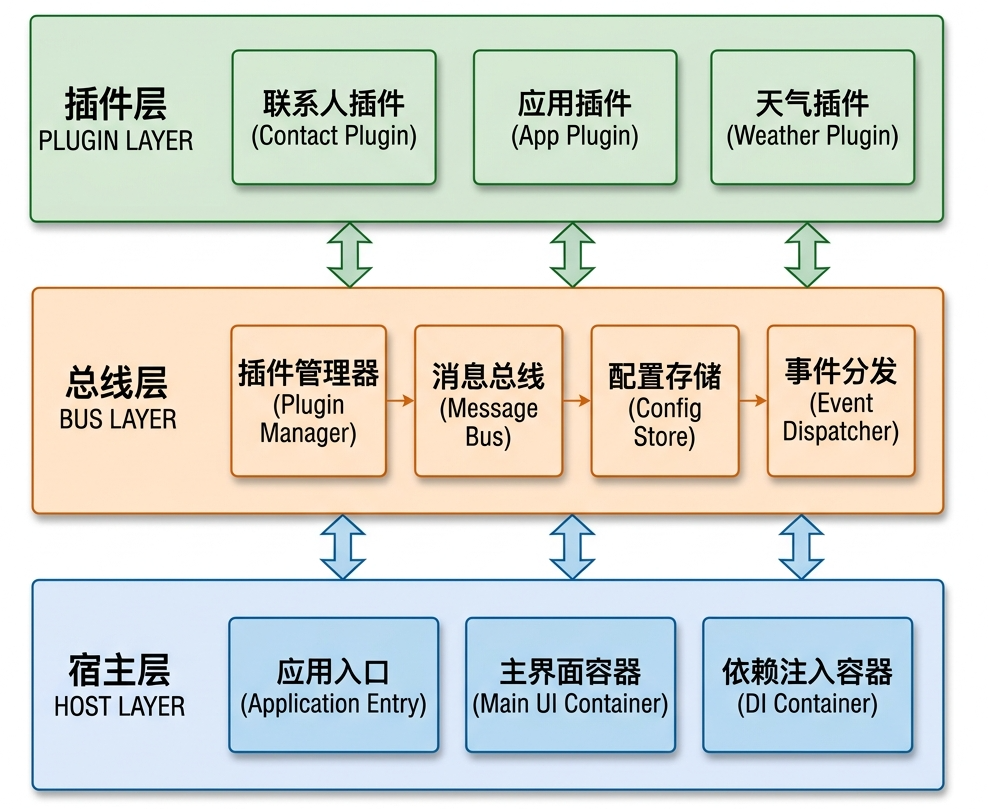
\includegraphics[width=0.82\textwidth]{figures/architecture.png}
    \caption{系统三层总体架构示意图}
    \label{fig:system_architecture}
\end{figure}


（1）宿主层：宿主层是整个系统的基础运行环境，由应用入口、主界面容器、依赖注入容器等组件构成。应用入口负责系统启动时的初始化工作，包括依赖注入容器的构建、插件系统的注册与启动、全局生命周期回调的注册等。主界面容器作为系统的Launcher入口，负责呈现适老化主屏，并管理与系统级广播的交互。依赖注入容器则统一管理整个应用中所有共享对象的创建和提供\upcite{24}。

宿主层的设计目标是为上层业务逻辑提供稳定可靠的运行环境，自身保持最小化、最简化，仅承担必要的基础设施职责，这与微内核架构中核心最小化的设计原则一脉相承\upcite{25}。

（2）总线层：总线层是系统中各功能模块之间通信协作的中枢，由插件管理器、消息总线、配置存储和事件分发四类核心组件构成。插件管理器统一管理所有插件的安装、启用、禁用和卸载操作，并维护插件运行状态的实时数据流，向界面层提供可视化管理能力。消息总线为不同插件之间的通信提供异步广播和点对点请求两种模式，确保模块协作既灵活又可靠。配置存储为每个插件分配独立的存储空间，避免不同插件的配置数据互相干扰。事件分发则负责将应用层的全局事件广播给所有关注该事件的插件。

总线层的引入将原本可能直接耦合的业务模块解耦为通过统一接口协作的独立单元，从而显著提升了系统的可维护性。

（3）插件层：插件层承载具体的业务功能，目前包含三个内置插件。联系人插件负责老年用户常用联系对象的存储管理，并提供电话直拨和微信视频/语音通话的发起能力。应用插件负责扫描设备已安装应用，维护用户自定义的常用应用列表，并提供桌面应用启动能力。天气插件负责通过开放天气接口获取实时天气信息，并将天气数据通过消息总线广播给关注的模块\upcite{28}。

每个插件遵循统一的生命周期规范，依次经历初始化、启动、运行、停止、销毁五个阶段，状态变迁通过状态机严格控制，以保证生命周期的可观察性和可控性。三个插件相互独立，单个插件的故障不会影响其他插件的正常运行，这一特性对适老化系统的稳定性意义重大。

\subsection{数据库设计}

系统的本地数据存储基于Room数据库实现\upcite{22}，主要包含联系人表与应用信息表两张核心数据表。联系人表用于存储老年用户的常用联系对象，主要字段包括联系人编号（主键）、姓名、电话号码、微信昵称、本地头像路径、显示顺序、是否支持视频通话、是否支持语音通话、是否支持电话拨号、创建时间、更新时间等。应用信息表用于存储设备上已扫描到的应用列表，主要字段包括应用包名（主键）、应用名称、图标二进制数据、是否启用、显示顺序、安装时间、最近更新时间等。

除Room数据库外，用户的全局设置（语音开关、字号档位、主题模式、对比度模式、网络守护开关、是否首次启动等）通过DataStore以键值对形式持久化存储\upcite{23}；插件级配置则采用每插件独立DataStore的隔离方案，避免跨插件的配置污染。

\section{功能模块设计与实现}

本系统围绕老年群体的核心诉求，在三层微内核架构的基础上，将具体业务解耦并划分为若干相互协作的功能模块。这些模块涵盖了适老化界面呈现、自动化直连通信、网络主动守护以及智能语音辅助等核心能力，共同构成了一个稳定、易用、安全的适老化系统。系统总体模块结构如下图所示：

\begin{figure}[htbp]
    \centering
    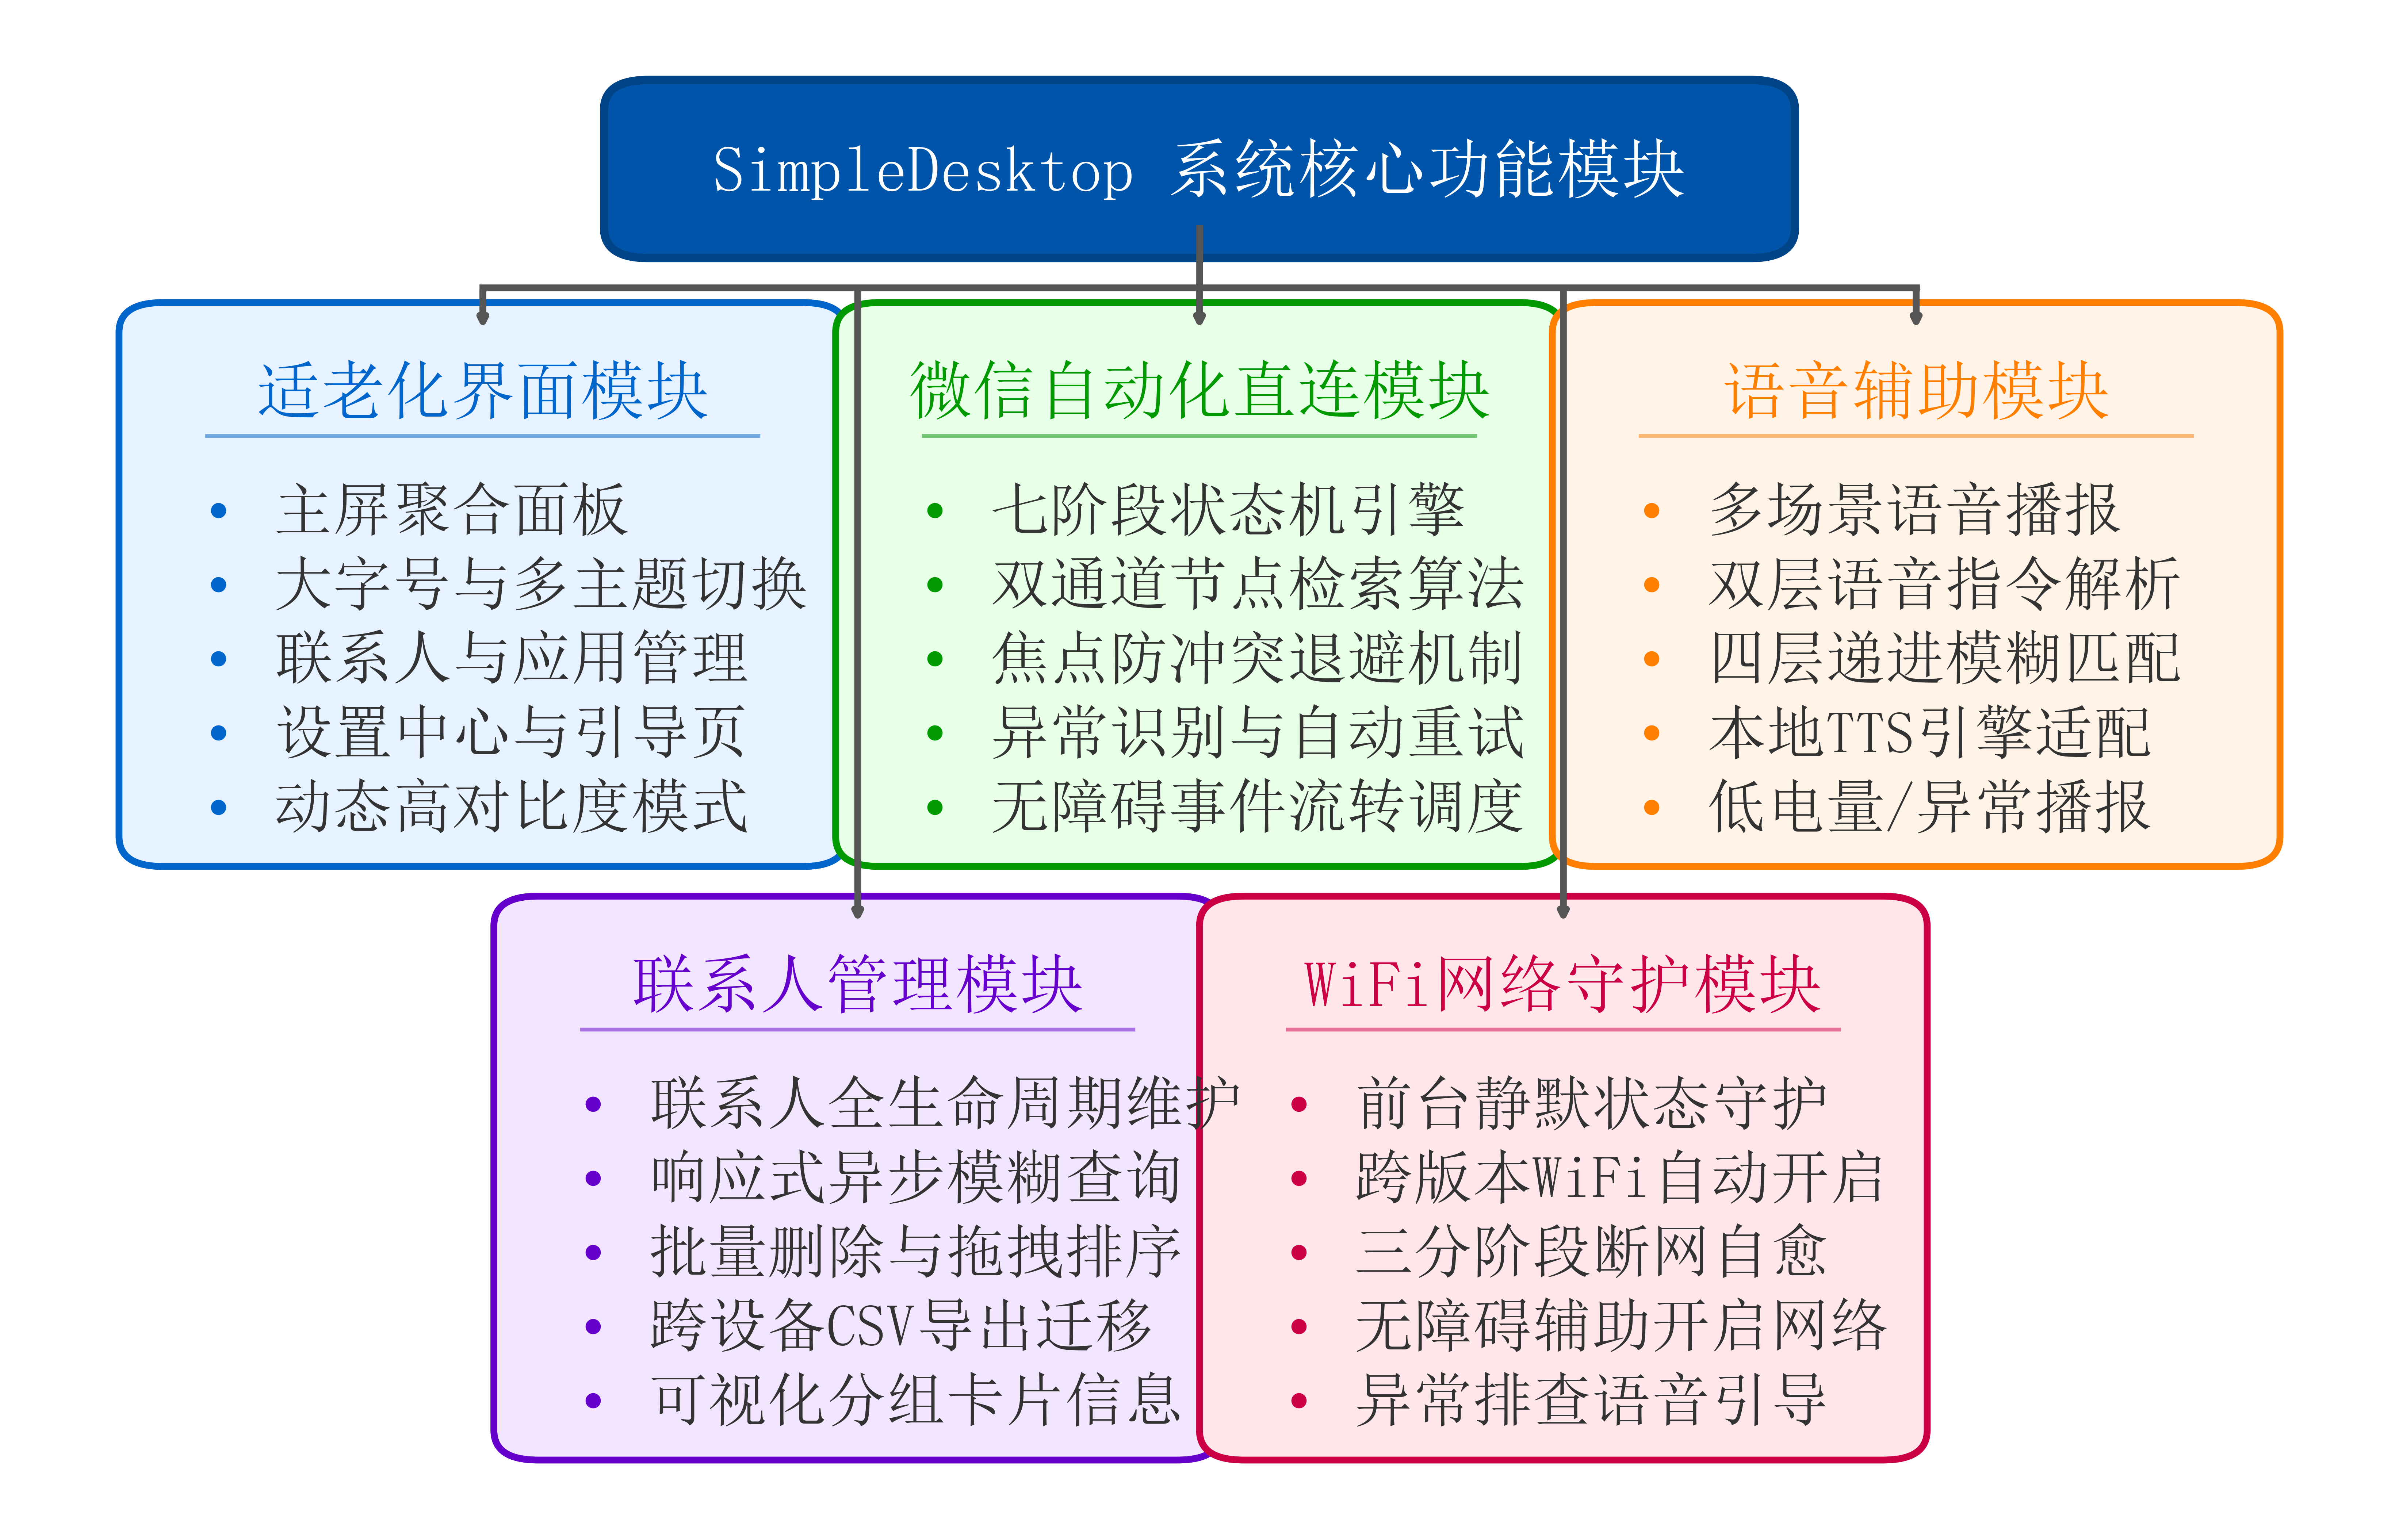
\includegraphics[width=\textwidth]{figures/fig3_1_system_modules.png}
    \caption{SimpleDesktop 适老桌面系统核心功能模块结构}
    \label{fig:system_modules}
\end{figure}


\subsection{开发环境}

本系统的开发与测试基于以下软硬件环境进行。开发主机选用搭载M系列处理器的MacBook Pro，操作系统为macOS 14.0。集成开发环境采用Android Studio Iguana（2023.2.1）正式版，构建工具为Gradle 8.6，编程语言为Kotlin 2.0.21，最低支持Android API 24（Android 7.0），目标API 34（Android 14），实际兼容性真机测试与适配覆盖了Android 14至Android 16的主流定制系统及HarmonyOS NEXT。版本控制采用Git结合Github代码托管平台。

系统所依赖的核心第三方库与版本如表3-1所示，涵盖了UI构建、依赖注入、数据持久化、网络请求、图片加载等关键能力。所有依赖均通过Gradle Version Catalog进行版本统一管理，确保依赖关系清晰可控。

\begin{table}[htbp]
  \centering
  \small
  \caption{主要开发依赖列表}
  \label{tab:development_dependencies}
  \renewcommand{\arraystretch}{1.3}
  \begin{threeparttable}
  \begin{tabular}{cll}
    \toprule
    \tableheader{序号} & \tableheader{模块层级} & \tableheader{依赖库与版本} \\
    \midrule
    \tablecell{1} & \tablecell{UI层} & \tablecell{Jetpack Compose 1.5.15、Material3、Compose Navigation\upcite{20,21}} \\
    \tablecell{2} & \tablecell{依赖注入} & \tablecell{Dagger-Hilt 2.56.2\upcite{24}} \\
    \tablecell{3} & \tablecell{数据持久化} & \tablecell{Room 2.6、DataStore Preferences\upcite{22,23}} \\
    \tablecell{4} & \tablecell{异步与响应式} & \tablecell{Kotlinx Coroutines\upcite{19}} \\
    \tablecell{5} & \tablecell{网络请求} & \tablecell{Retrofit 2 + OkHttp + Gson} \\
    \tablecell{6} & \tablecell{图片加载} & \tablecell{Coil} \\
    \tablecell{7} & \tablecell{权限管理} & \tablecell{XXPermissions} \\
    \tablecell{8} & \tablecell{农历计算} & \tablecell{Lunar Java库} \\
    \bottomrule
  \end{tabular}
  \end{threeparttable}
\end{table}


测试环境则覆盖多型号、多分辨率、多Android版本的真机环境，详细测试设备清单将在第4章测试章节中予以介绍。

\subsection{适老化界面模块}

（1）模块功能概述：
适老化界面模块负责构建符合老年用户视觉与认知特征的桌面交互界面，是用户与系统交互的第一接触面。模块主要包含主屏聚合面板、联系人管理界面、应用管理界面、设置中心、引导页、权限管理等子界面。

（2）主屏聚合面板设计：
主屏作为老年用户最频繁访问的界面，采用了卡片化的聚合面板设计。屏幕顶部为大尺寸时间天气信息卡，集中呈现实时时间（数字时钟，每秒刷新）、日期、星期、农历、天气图标、温度等高频信息。中部为两列卡片网格区，第一行预置手电筒卡片和语音助手卡片两个高频功能入口，第二行起依次平铺常用联系人卡片和常用应用卡片。整体布局遵循上信息、中操作、下扩展的视觉层次，老年用户无需滑动或跳转便可触达绝大多数日常操作入口。

（3）字号与主题动态切换：
考虑到不同老年用户对字号的偏好存在差异，系统提供小、中、大三档字号方案，每档对应一套完整的字号定义（涵盖标题、正文、说明文字等共15种字体角色）。当用户在设置中切换字号档位时，对应的字号配置通过响应式数据流向上传播，整个应用界面在下一帧自动按新字号重组刷新，无需重启应用。

主题模式上，系统提供经典蓝与暖心橙两套色彩方案。前者强调专业、冷静、稳重的视觉感受，后者突出温暖、亲切、活力的氛围，老年用户可根据个人喜好自由选择。此外系统还提供高对比度模式，将界面切换为黑底白字的高对比方案，特别适合视力较弱的老年用户。

（4）实现要点：
适老化界面模块基于Jetpack Compose声明式UI框架构建\upcite{20}。所有界面元素均通过可组合函数描述，状态由视图模型托管，主题、字号、对比度等全局参数通过Compose的CompositionLocal机制向下传递，确保整个组件树的一致性。列表类界面（如联系人列表、应用列表）采用LazyVerticalGrid组件实现惰性加载，仅渲染屏幕可见范围内的条目，保证大数据量下的滑动流畅性。

\subsection{微信自动化直连模块}
（1）模块功能概述：微信自动化直连模块是本系统的核心创新功能。其目标是将微信视频通话原本需要七步操作的流程，简化为老年用户在桌面上的一次点击。从用户视角看，老年用户只需点击桌面联系人卡片，在弹出的简洁面板中选择视频通话或语音通话，系统便自动完成微信内部所有后续操作并一步一步进入通话界面。

（2）业务流程难点分析：一键直拨方案的实现面临四方面难点。第一，目标应用界面不可控。微信作为第三方应用，其内部界面随版本迭代频繁变化，控件标识符可能因代码混淆或原生架构变动而失去稳定性\upcite{17}。第二，操作时序难以预测。微信内部页面切换的耗时受设备性能、网络状况等因素影响显著，过早或过晚的操作都可能导致流程失败。第三，外部干扰难以避免。在自动化流程执行过程中，可能突然出现来电通知、系统弹窗等外部干扰，导致焦点离开微信界面。第四，部分操作需要特殊处理。微信功能菜单中的通话选项不一定支持标准的点击事件触发，需要采用模拟手势的方式进行触发。

（3）七阶段状态机设计：针对上述难点，本模块将微信视频通话的自动化流程建模为一个七阶段的状态机\upcite{16}。状态机的设计借鉴了通信工程领域有限状态机模型的成熟思想，将复杂的动态过程分解为有限个相对独立、可观察、可验证、可重试的状态。


阶段一为微信主界面就位阶段。状态机检查当前活动窗口是否为微信主界面，若是则点击底部第一个标签页确保停留在聊天列表，若不是则通过系统返回操作逐步退回，直至到达主界面。

阶段二为搜索入口触发阶段。状态机定位主界面顶部的搜索图标并执行点击操作，使界面进入搜索页面。

阶段三为联系人姓名输入阶段。状态机定位搜索页面的输入框并将目标联系人的微信昵称写入，然后等待短暂的搜索响应时间。

阶段四为搜索结果确认阶段。状态机在搜索结果列表中点击与目标联系人匹配的条目，进入聊天界面。

阶段五为聊天功能展开阶段。状态机定位聊天界面右下方的功能菜单按钮并执行点击操作。

阶段六为通话选项选择阶段。状态机在展开的功能菜单中定位通话相关菜单项，并通过模拟手势方式在菜单项的中心坐标执行点击。

阶段七为通话类型确认阶段。如果上一阶段触发了通话类型选择弹窗，状态机进一步在弹窗中点击与用户偏好一致的通话方式选项，完成全部自动化流程后将状态机阶段索引重置为初始值。

\begin{figure}[!ht]
  \centering
  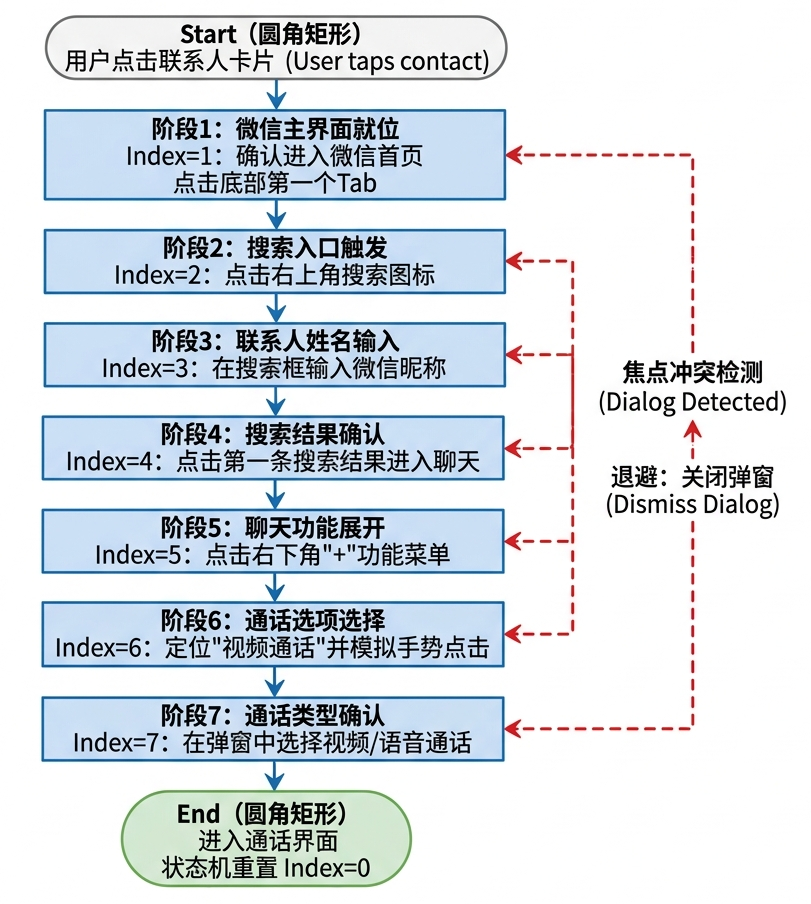
\includegraphics[width=0.6\textwidth]{figures/wechat_state.png}
  \caption{微信一键直拨七阶段状态机流程}
  \label{fig:wechat_state_machine}
\end{figure}

七个阶段之间通过事件驱动加状态推进的方式协作。每个阶段在自身操作完成后等待数百毫秒至一秒不等的时间，使界面切换得以完成，然后将状态机阶段索引推进至下一阶段。下一次窗口状态变化或内容变化事件被触发时，状态机便在新的界面上继续执行下一阶段。



（4）双通道节点检索算法：为应对微信版本更新带来的控件标识符变化问题，本模块设计了双通道节点检索算法\upcite{17}。算法的核心思想是同时利用控件标识符和文本内容两类不同性质的信息进行节点定位，在主通道失效时自动切换到备用通道。

在每次需要定位界面节点时，算法首先尝试通过控件标识符查找节点。这一通道使用控件树的标识符索引，时间复杂度极低，在标识符稳定时能够快速准确地命中目标。如果通过控件标识符未能找到目标节点，算法立即切换到第二通道，通过文本内容进行查找。第二通道遍历控件树查找匹配文本的节点，虽然时间复杂度相对较高，但具备良好的稳定性。

双通道协同的设计将高效与稳健有机结合：在通常情况下系统享受第一通道带来的高效执行，在异常情况下又能依靠第二通道避免完全失败。实测在微信8.0.30到最新版本的多个版本上，整体流程成功率均保持在99.1\%以上，平均流程耗时为5至6秒。

（5）焦点防冲突退避机制：焦点冲突是指自动化流程预期操作的目标窗口与实际处于活动状态的窗口不一致的情况。当焦点冲突发生时，无障碍服务读取到的活动窗口节点树将不再属于微信主界面，而属于干扰窗口，可能导致流程失败甚至产生意外行为\upcite{13}。

针对焦点冲突，本模块设计了识别异常、主动退避、等待恢复、自动重试的退避策略。无障碍服务在每次接收到事件时，检查当前活动窗口的类名是否包含典型的对话框关键字。一旦检测到对话框存在，便立即通过系统返回操作主动关闭对话框。退避操作完成后，状态机不推进到下一阶段，而是保持在当前阶段等待下一次窗口事件触发。整个退避、恢复、重试过程对老年用户完全透明，用户只会感觉到流程稍有延迟但最终成功完成。

\subsection{WiFi网络守护模块}

WiFi是老年用户语音通话、视频连线的核心通信保障，其稳定性直接影响系统可用性。

（1）模块功能概述：WiFi网络守护模块旨在解决老年用户因误触WiFi开关或路由器信号波动导致的网络异常问题，确保终端通信链路的连续性。模块由前台守护服务、网络回调监听、WiFi自动开启无障碍服务、用户引导面板四部分组成，形成完整的检测、等待、自愈、引导闭环。

（2）前台守护服务：为实现网络状态的持续监测，模块采用前台服务模式运行后台守护逻辑。前台服务通过在系统通知栏显示一条低优先级、静默模式的常驻通知向操作系统表明服务的活跃性，从而获得较高的进程保活优先级。服务启动后立即向系统的连接管理器注册WiFi类型的网络回调监听，实时感知WiFi连接状态变化。

（3）基于无障碍服务的WiFi自动开启：由于系统安全性与隐私保护设计，自 Android 10及以上版本起（本系统实际测试覆盖的Android 14至16均适用），操作系统不再允许应用通过编程接口直接控制WiFi开关。因此，本模块统一采用无障碍服务辅助开启的方案：当检测到网络异常需要开启WiFi时，模块设置无障碍服务的工作标志位，并主动跳转到系统WiFi设置页面；专门设计的WiFi自动开启无障碍服务监听设置页面的事件，自动定位并点击WiFi开关，操作完成后通过模拟Home键返回桌面。整个过程对老年用户完全透明\upcite{13}。整个守护与自愈的详细流程机制如下图所示：

\begin{figure}[h]
  \centering
  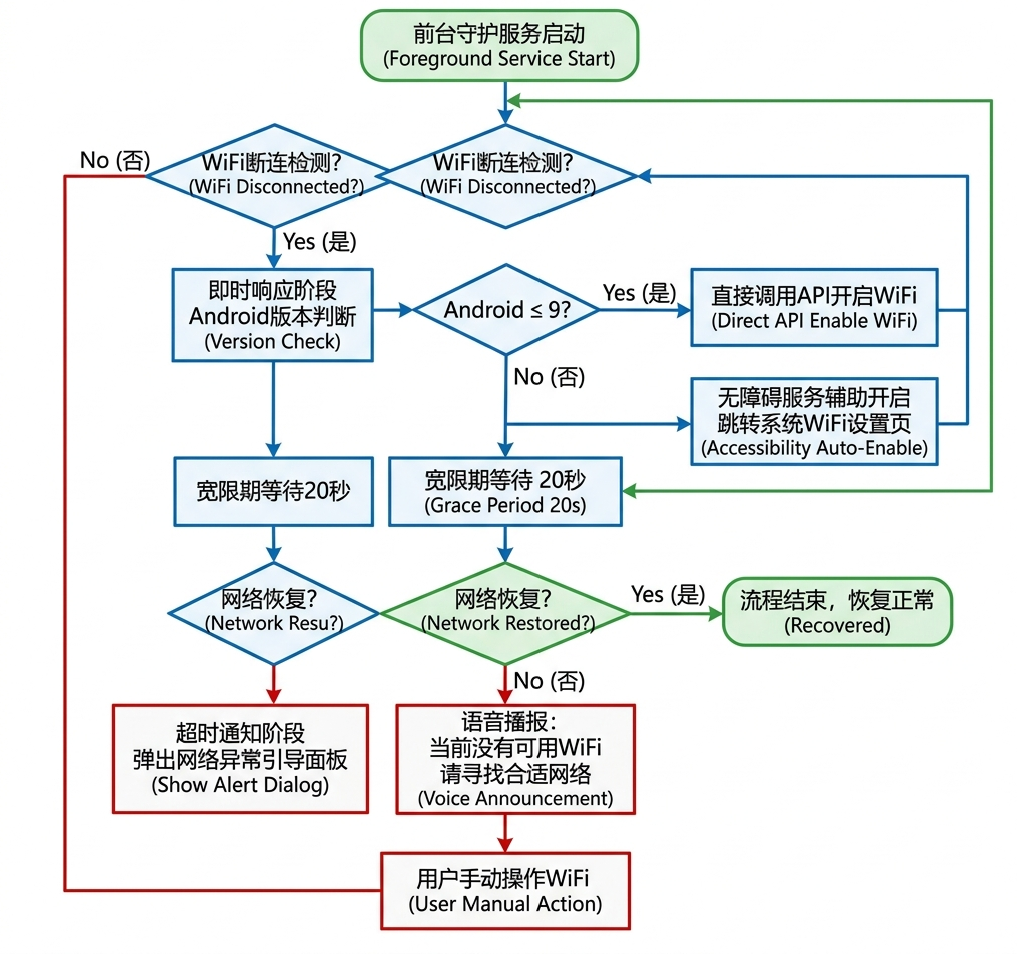
\includegraphics[width=1.0\textwidth]{figures/wifi_daemon.png}
  \caption{WiFi网络守护与自愈机制流程}
  \label{fig:wifi_daemon}
\end{figure}

（4）断网自愈与引导面板：断网自愈策略由即时响应、宽限等待、超时通知三个阶段构成。即时响应阶段在断连事件发生瞬间立即调用WiFi自动开启逻辑；宽限等待阶段给系统留出充分的恢复时间，期间持续监测网络状态，一旦连接恢复立即结束自愈流程；超时通知阶段在宽限期结束仍未恢复时，通过广播触发界面层的网络异常提示弹窗，并由语音助手播报“无可用网络”的语音提示，引导老年用户进行下一步操作。

网络异常提示弹窗采用大尺寸卡片式布局设计，主标题以醒目的字号和颜色呈现无可用WiFi网络，副标题以适中字号补充说明请寻找合适的网络连接，底部提供清晰的操作按钮。点击打开WiFi设置按钮后，系统直接跳转到Android的WiFi设置面板，老年用户完成WiFi连接后可直接返回桌面。

\subsection{语音辅助模块}

（1）模块功能概述：语音辅助模块由语音播报与语音指令解析两个子模块组成，旨在为视力不佳或不擅长触屏操作的老年用户提供听觉通道与语音通道的辅助交互。

\begin{figure}[htbp]
  \centering
  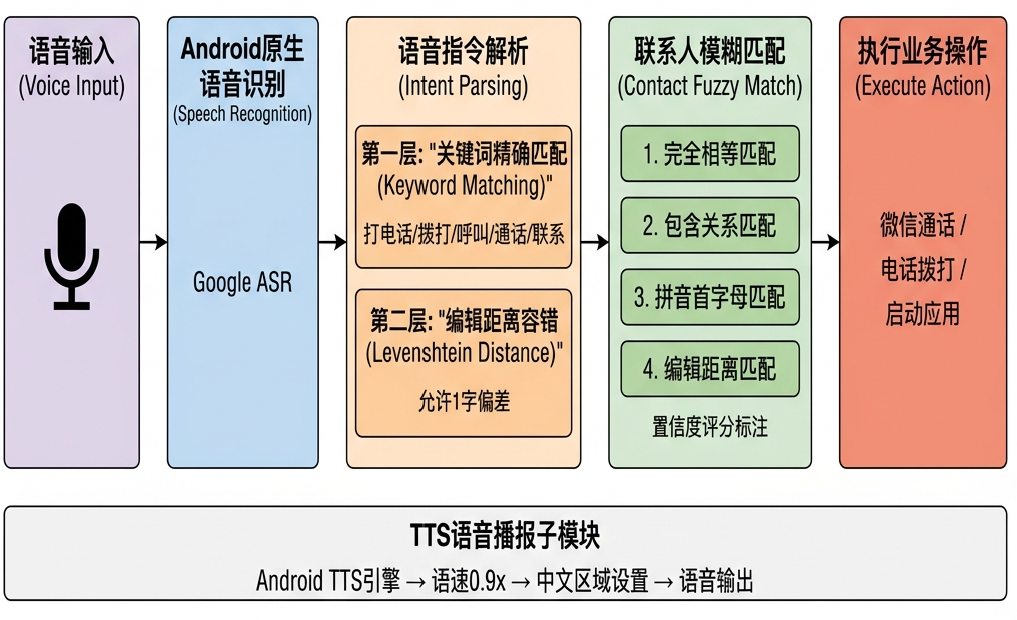
\includegraphics[width=1.0\textwidth]{figures/voice_flow.png}
  \caption{语音辅助模块工作流程}
  \label{fig:voice_assistant_flow}
\end{figure}


（2）语音播报子模块：语音播报基于Android原生的文本转语音引擎封装实现，提供统一的语音播报接口，覆盖网络异常提示、操作执行确认、低电量提醒等多个使用场景。模块在初始化时尝试多种中文区域设置，以兼容不同手机厂商TTS引擎对中文支持的差异；语速默认设置为正常速度的0.9倍，使语音节奏更适合老年人的听觉接受能力。


（3）语音指令解析子模块：语音指令解析采用关键词匹配加编辑距离容错的轻量级双层策略\upcite{18}。第一层为关键词精确匹配，模块为每种支持的动作类型（包括打电话、打开应用、开关手电筒等）维护一组对应的关键词库（如打电话动作的关键词包括打电话、拨打、呼叫、通话、联系等十余个），通过遍历检查输入文本中是否包含某个关键词来识别用户意图。

第二层为编辑距离容错匹配，主要应对老年人发音不标准或语音识别引擎识别误差的情况。算法对输入文本中与关键词等长的每个子串计算与该关键词的编辑距离，允许一个字符的偏差即视为匹配。这种容错机制使系统在面对识别误差时依然能够正确理解用户意图。

（4）联系人模糊匹配：在识别出打电话动作意图后，系统还需要将用户说出的联系人名称与通讯录中的实际联系对象进行匹配。模块采用四层递进的联系人模糊匹配策略：完全相等匹配、包含关系匹配、拼音首字母匹配和编辑距离匹配\upcite{18}，每一层匹配赋予不同的置信度评分。系统从最严格的完全相等匹配开始尝试，逐层放宽至最宽松的编辑距离匹配，并最终选择置信度最高且超过预设阈值的匹配结果作为目标联系人。



\subsection{联系人管理模块}
（1）模块功能概述：联系人管理模块为老年用户提供常用联系对象的全生命周期管理能力，覆盖联系人的新增、查询、修改、删除、排序、导出等核心功能，是支撑通讯类业务的基础数据模块。

（2）联系人新增与编辑：联系人新增界面采用分组卡片式布局，依次包含基本信息组（姓名、电话号码、微信昵称）、头像组（支持从相册选择或现场拍照）和通话能力组（视频通话、语音通话、电话直拨三个开关）。所有输入控件均采用大字号、宽边距设计，方便老年用户的视觉辨识与触摸操作。

联系人编辑界面与新增界面布局一致，区别在于初始数据由数据库回填，用户可直接修改现有信息。保存操作通过响应式数据流自动同步到数据库与主屏。

（3）联系人查询：联系人查询支持按姓名进行模糊搜索。用户在搜索框中输入任意关键字后，系统在协程中异步执行数据库的LIKE查询，并将结果通过Flow实时推送到界面层\upcite{19}。配合Compose的状态收集机制，搜索结果在用户输入的同时即时呈现，无需点击搜索按钮。

（4）联系人删除与排序：联系人删除支持单条删除与批量删除两种模式。为防止老年用户误操作，删除前系统弹出确认对话框，明确告知删除将不可撤销。

联系人排序由分配排序索引字段实现。用户可通过拖拽方式手动调整联系人在主屏上的显示顺序，新顺序通过协程异步写入数据库后立即反映到界面。

（5）联系人导出：为方便老年用户在更换设备时迁移联系人数据，系统提供联系人导出功能。导出格式为标准CSV文本文件，包含全部联系人字段，文件保存在设备的下载目录，可通过微信、邮件等渠道分享给子女进行备份。

\section{软件操作流程}

\subsection{首次启动与初始化流程}
用户首次安装并启动SimpleDesktop后，系统进入引导页流程。引导页通过左右滑动的方式依次介绍系统的核心功能特点（适老化界面、一键通话、网络守护、语音助手），帮助老年用户或其家属快速建立对系统能力的整体认知。


\begin{figure}[H]
    \centering
    \begin{minipage}{0.22\textwidth}
        \centering
        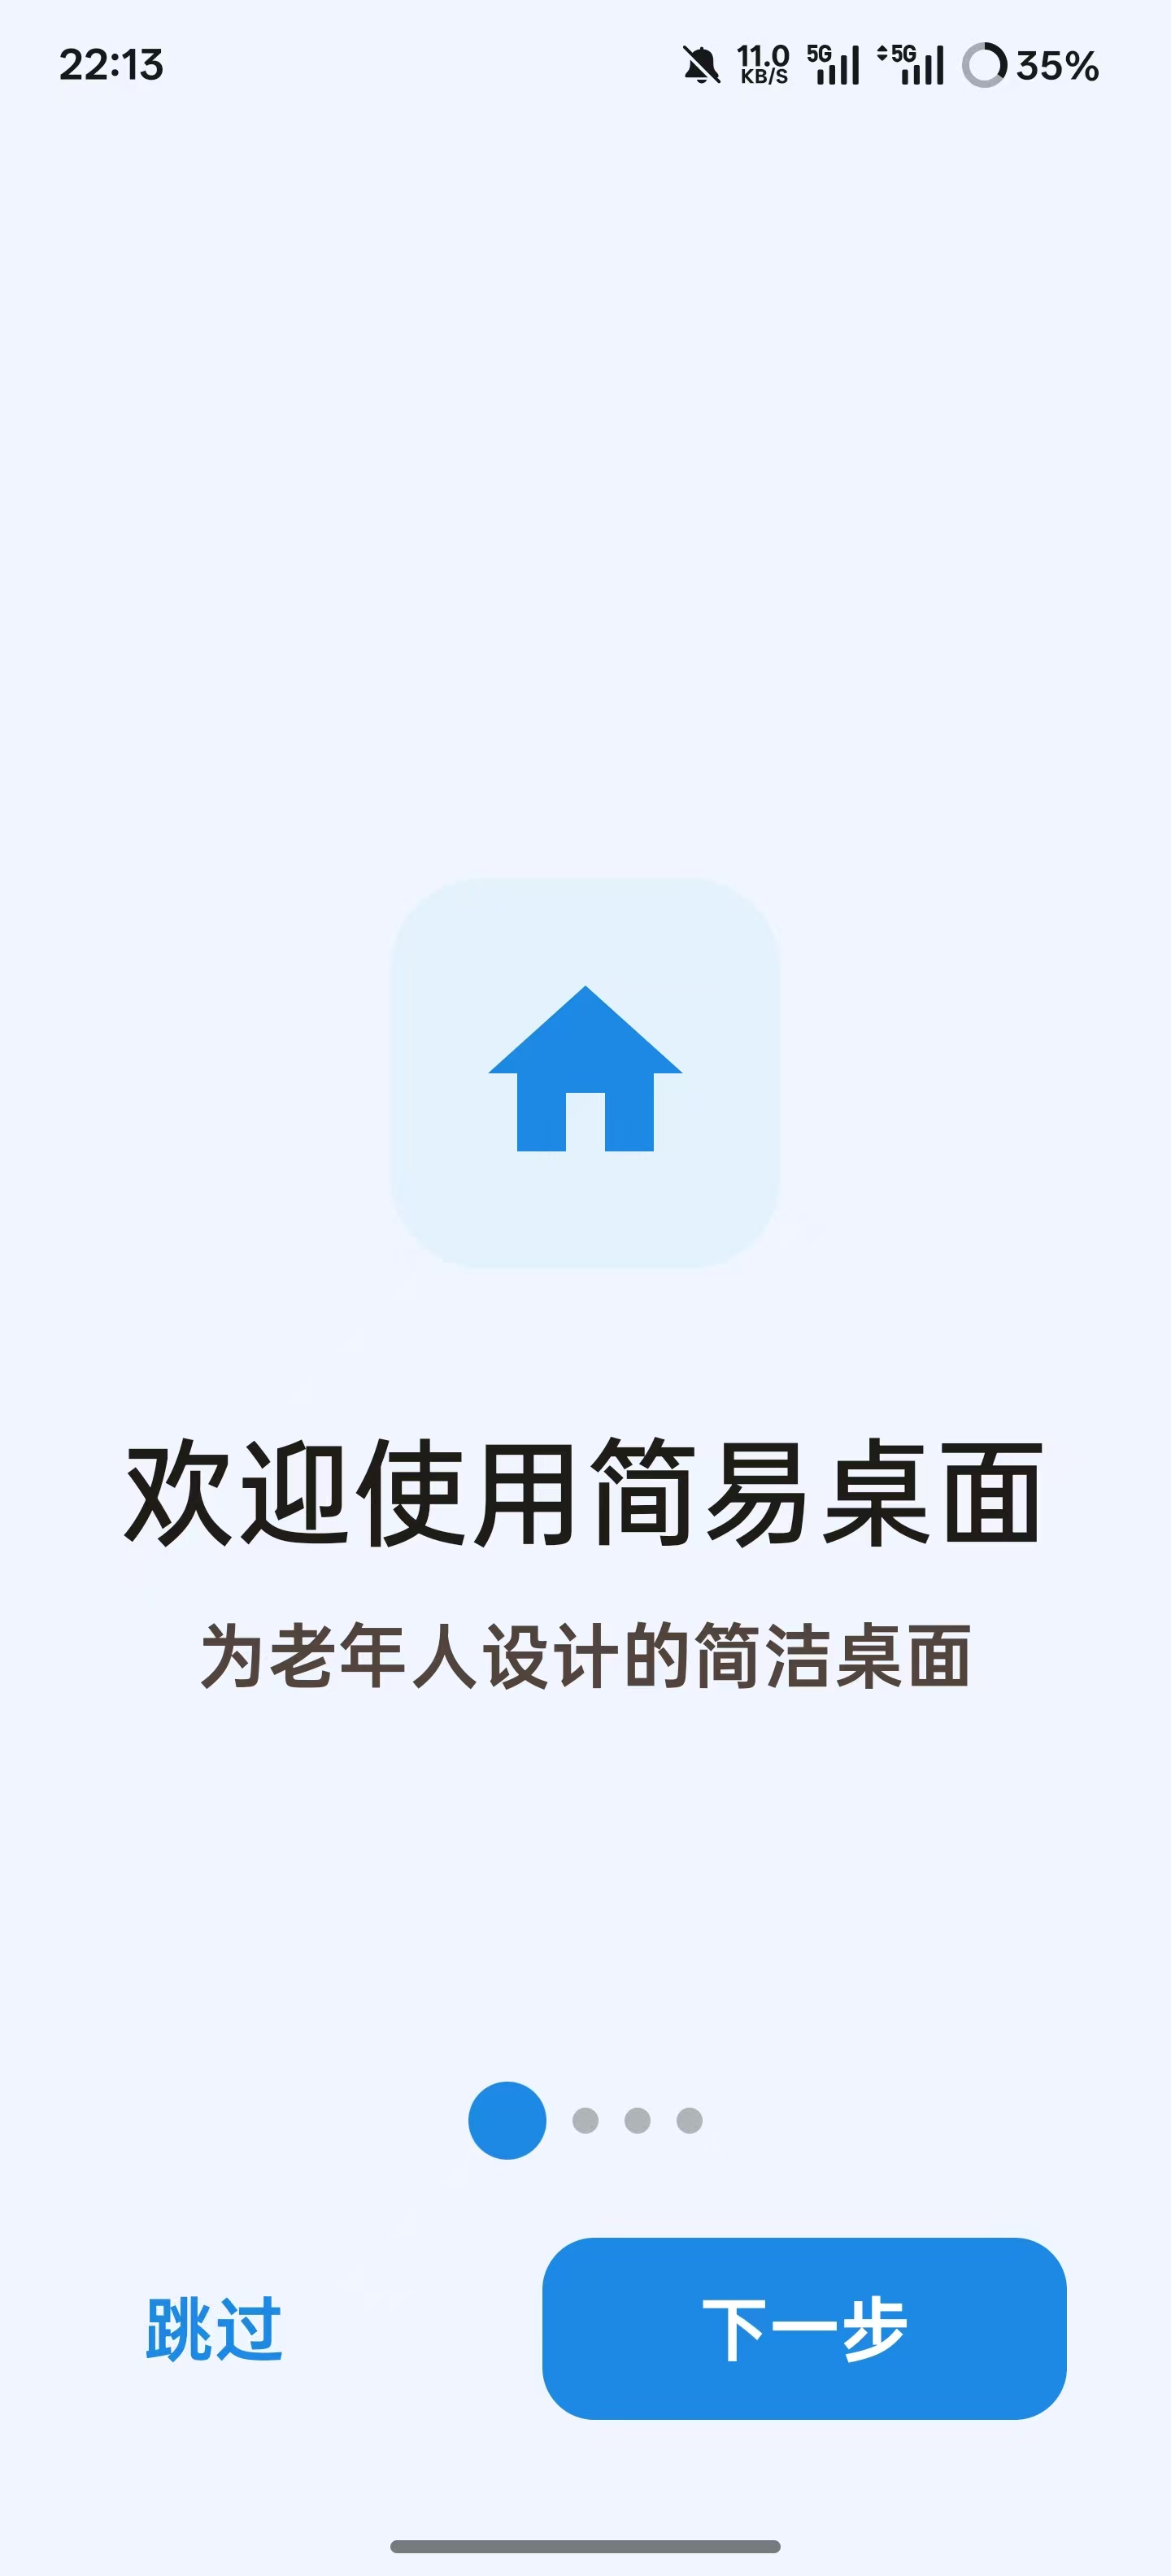
\includegraphics[width=\linewidth]{figures/wechat/desktop1.jpg}
        \caption*{(a) 首次启动}
    \end{minipage}\hfill
    \begin{minipage}{0.22\textwidth}
        \centering
        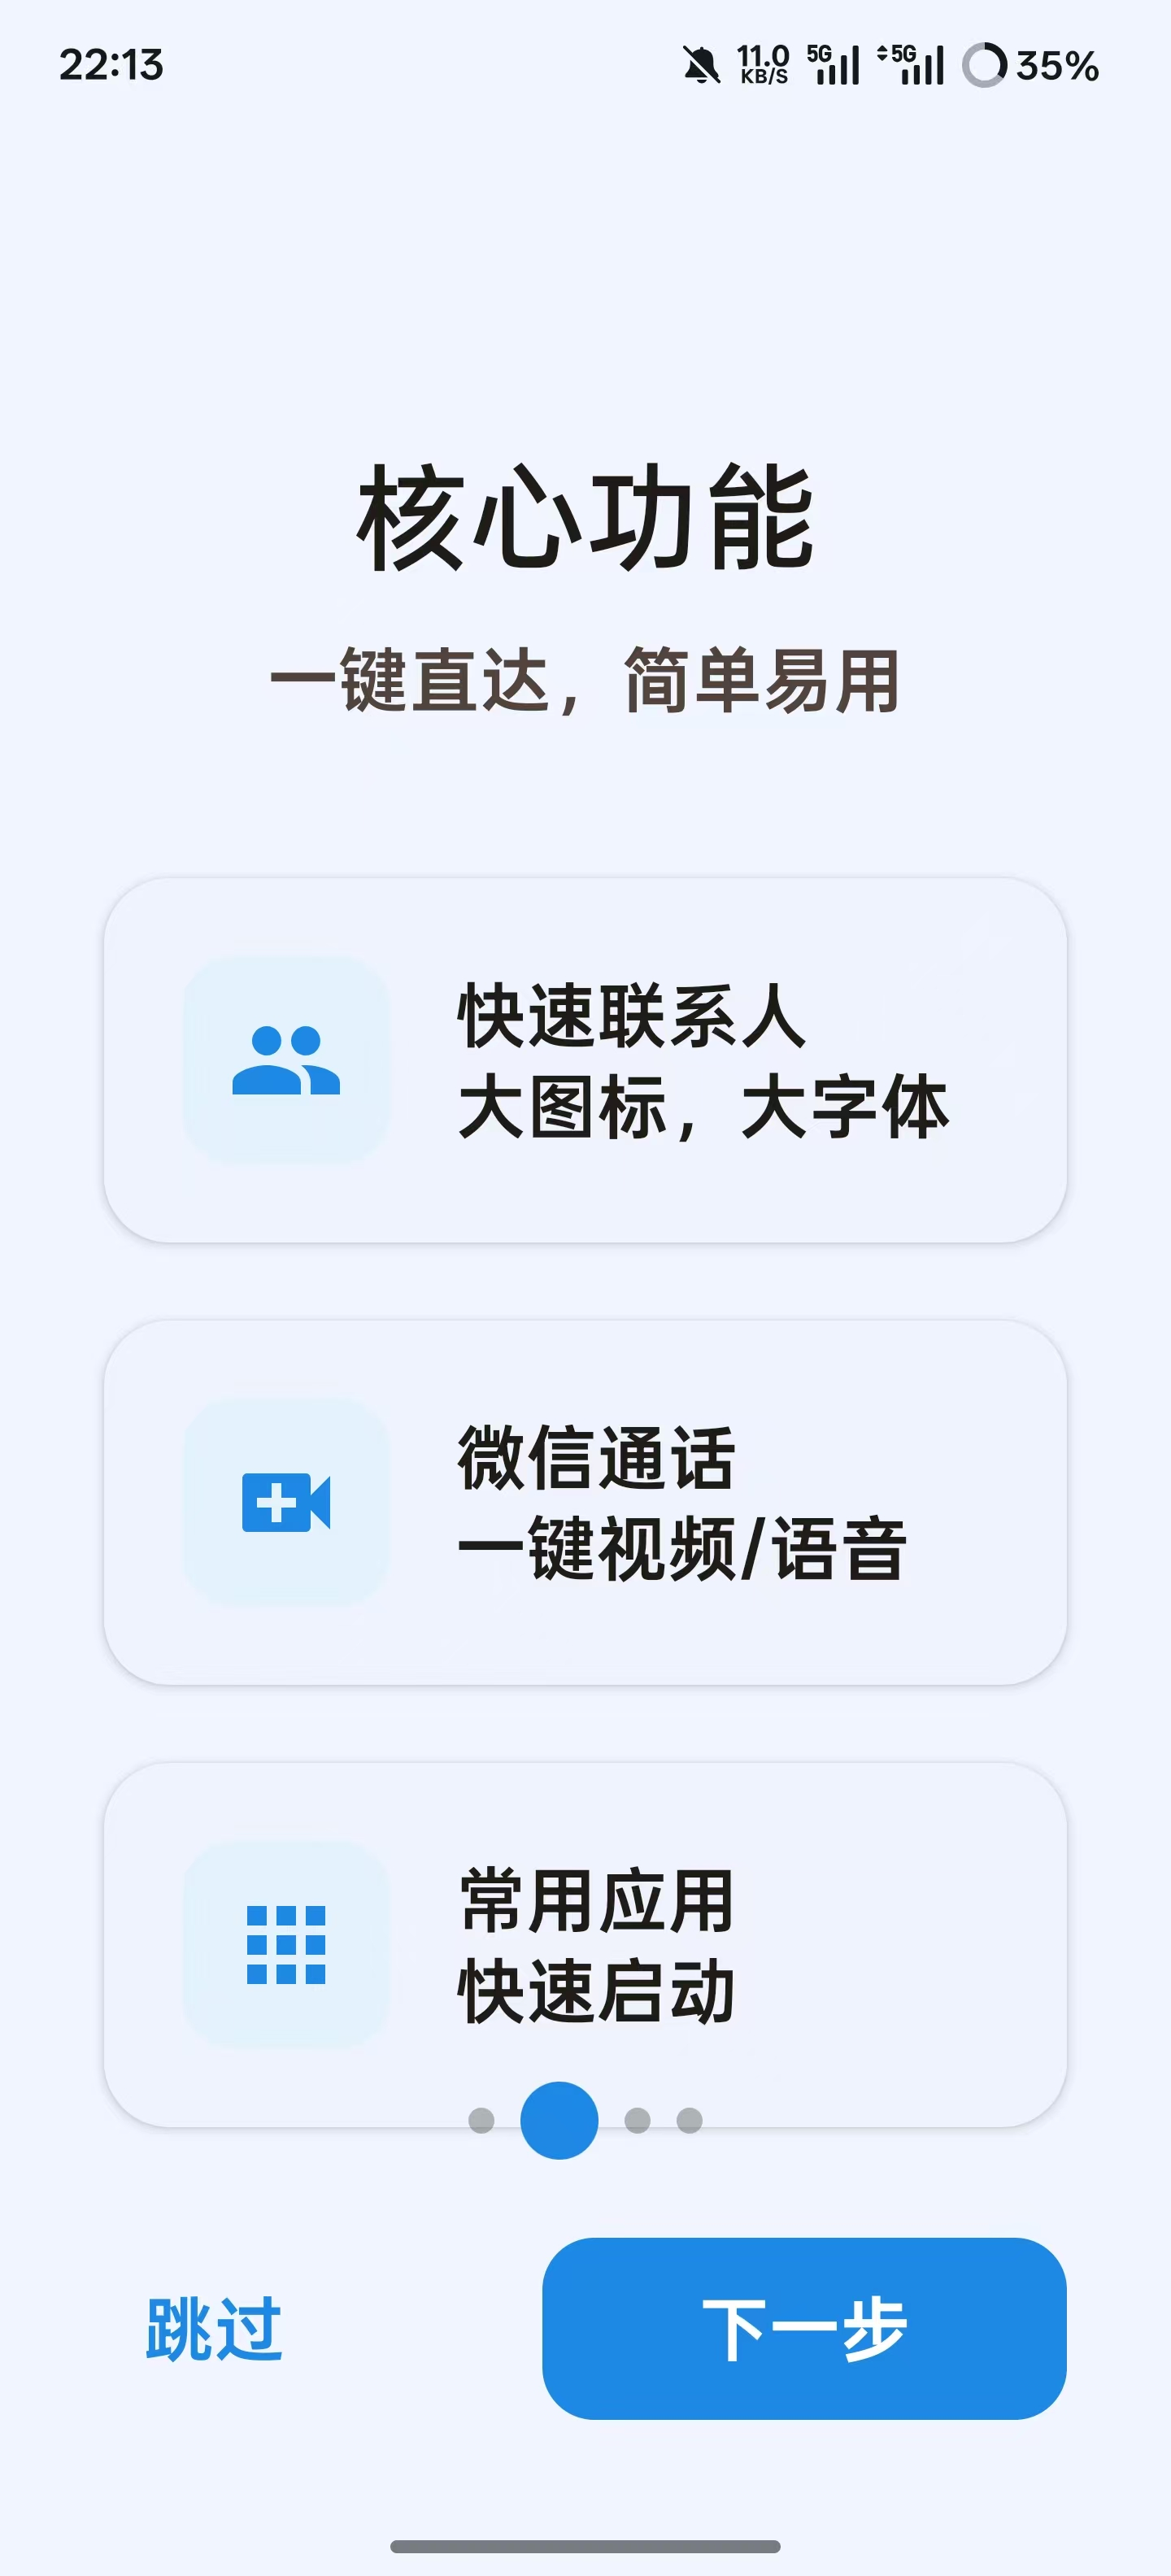
\includegraphics[width=\linewidth]{figures/wechat/desktop2.jpg}
        \caption*{(b) 功能介绍}
    \end{minipage}\hfill
    \begin{minipage}{0.22\textwidth}
        \centering
        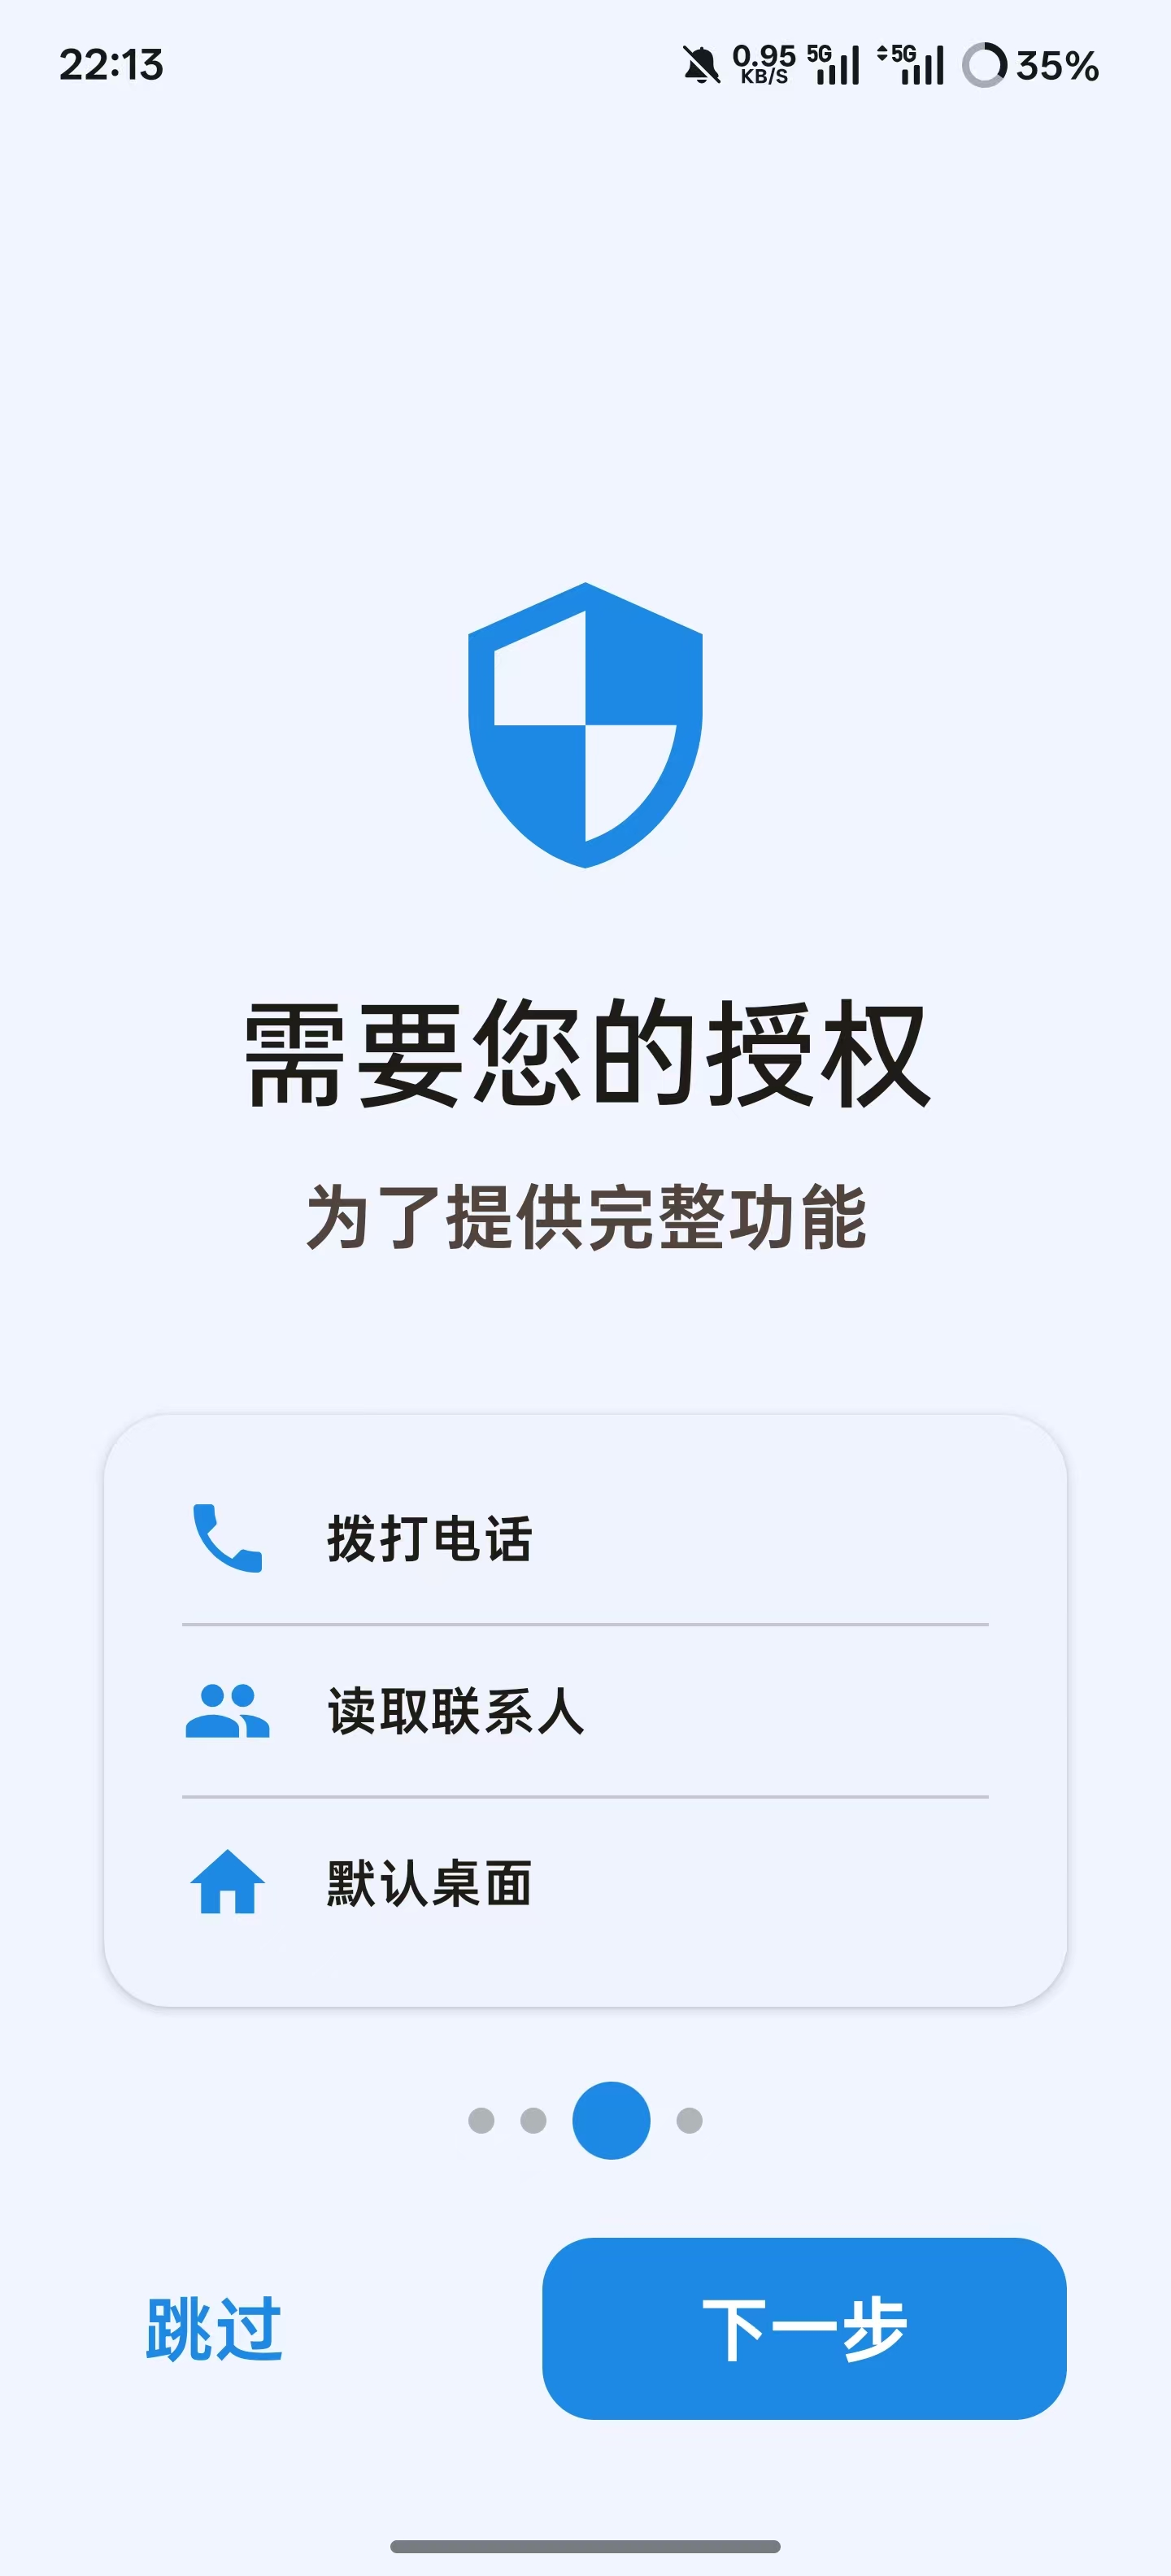
\includegraphics[width=\linewidth]{figures/wechat/desktop3.jpg}
        \caption*{(c) 权限授权}
    \end{minipage}

    \vspace{0.3cm}

    \begin{minipage}{0.22\textwidth}
        \centering
        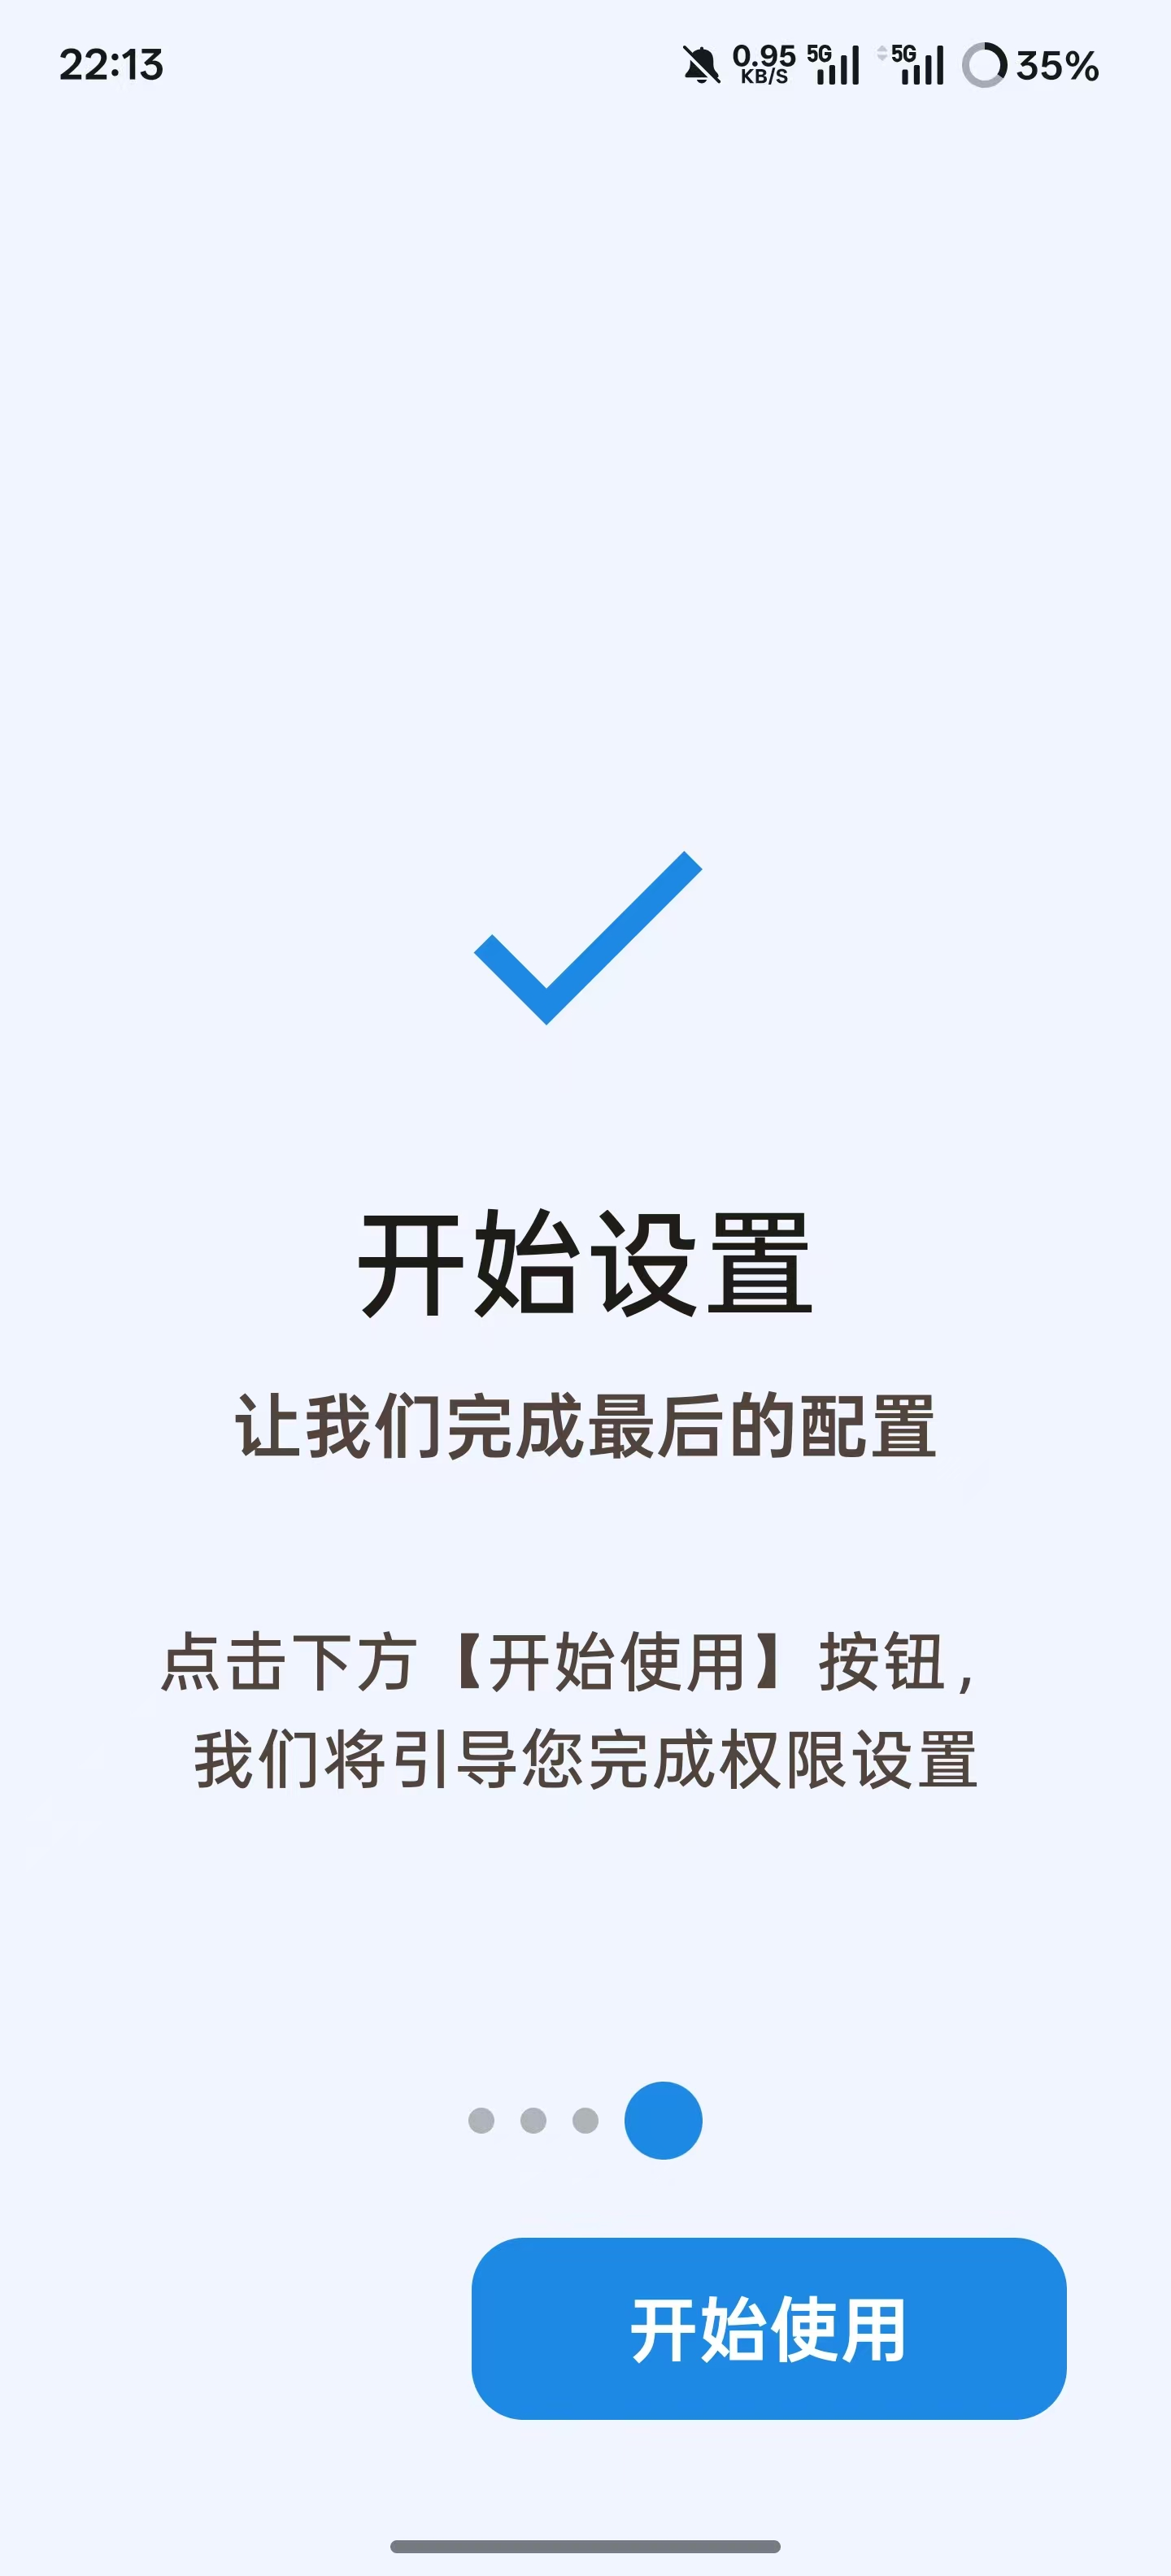
\includegraphics[width=\linewidth]{figures/wechat/desktop4.jpg}
        \caption*{(d) 开始设置}
    \end{minipage}\hfill
    \begin{minipage}{0.22\textwidth}
        \centering
        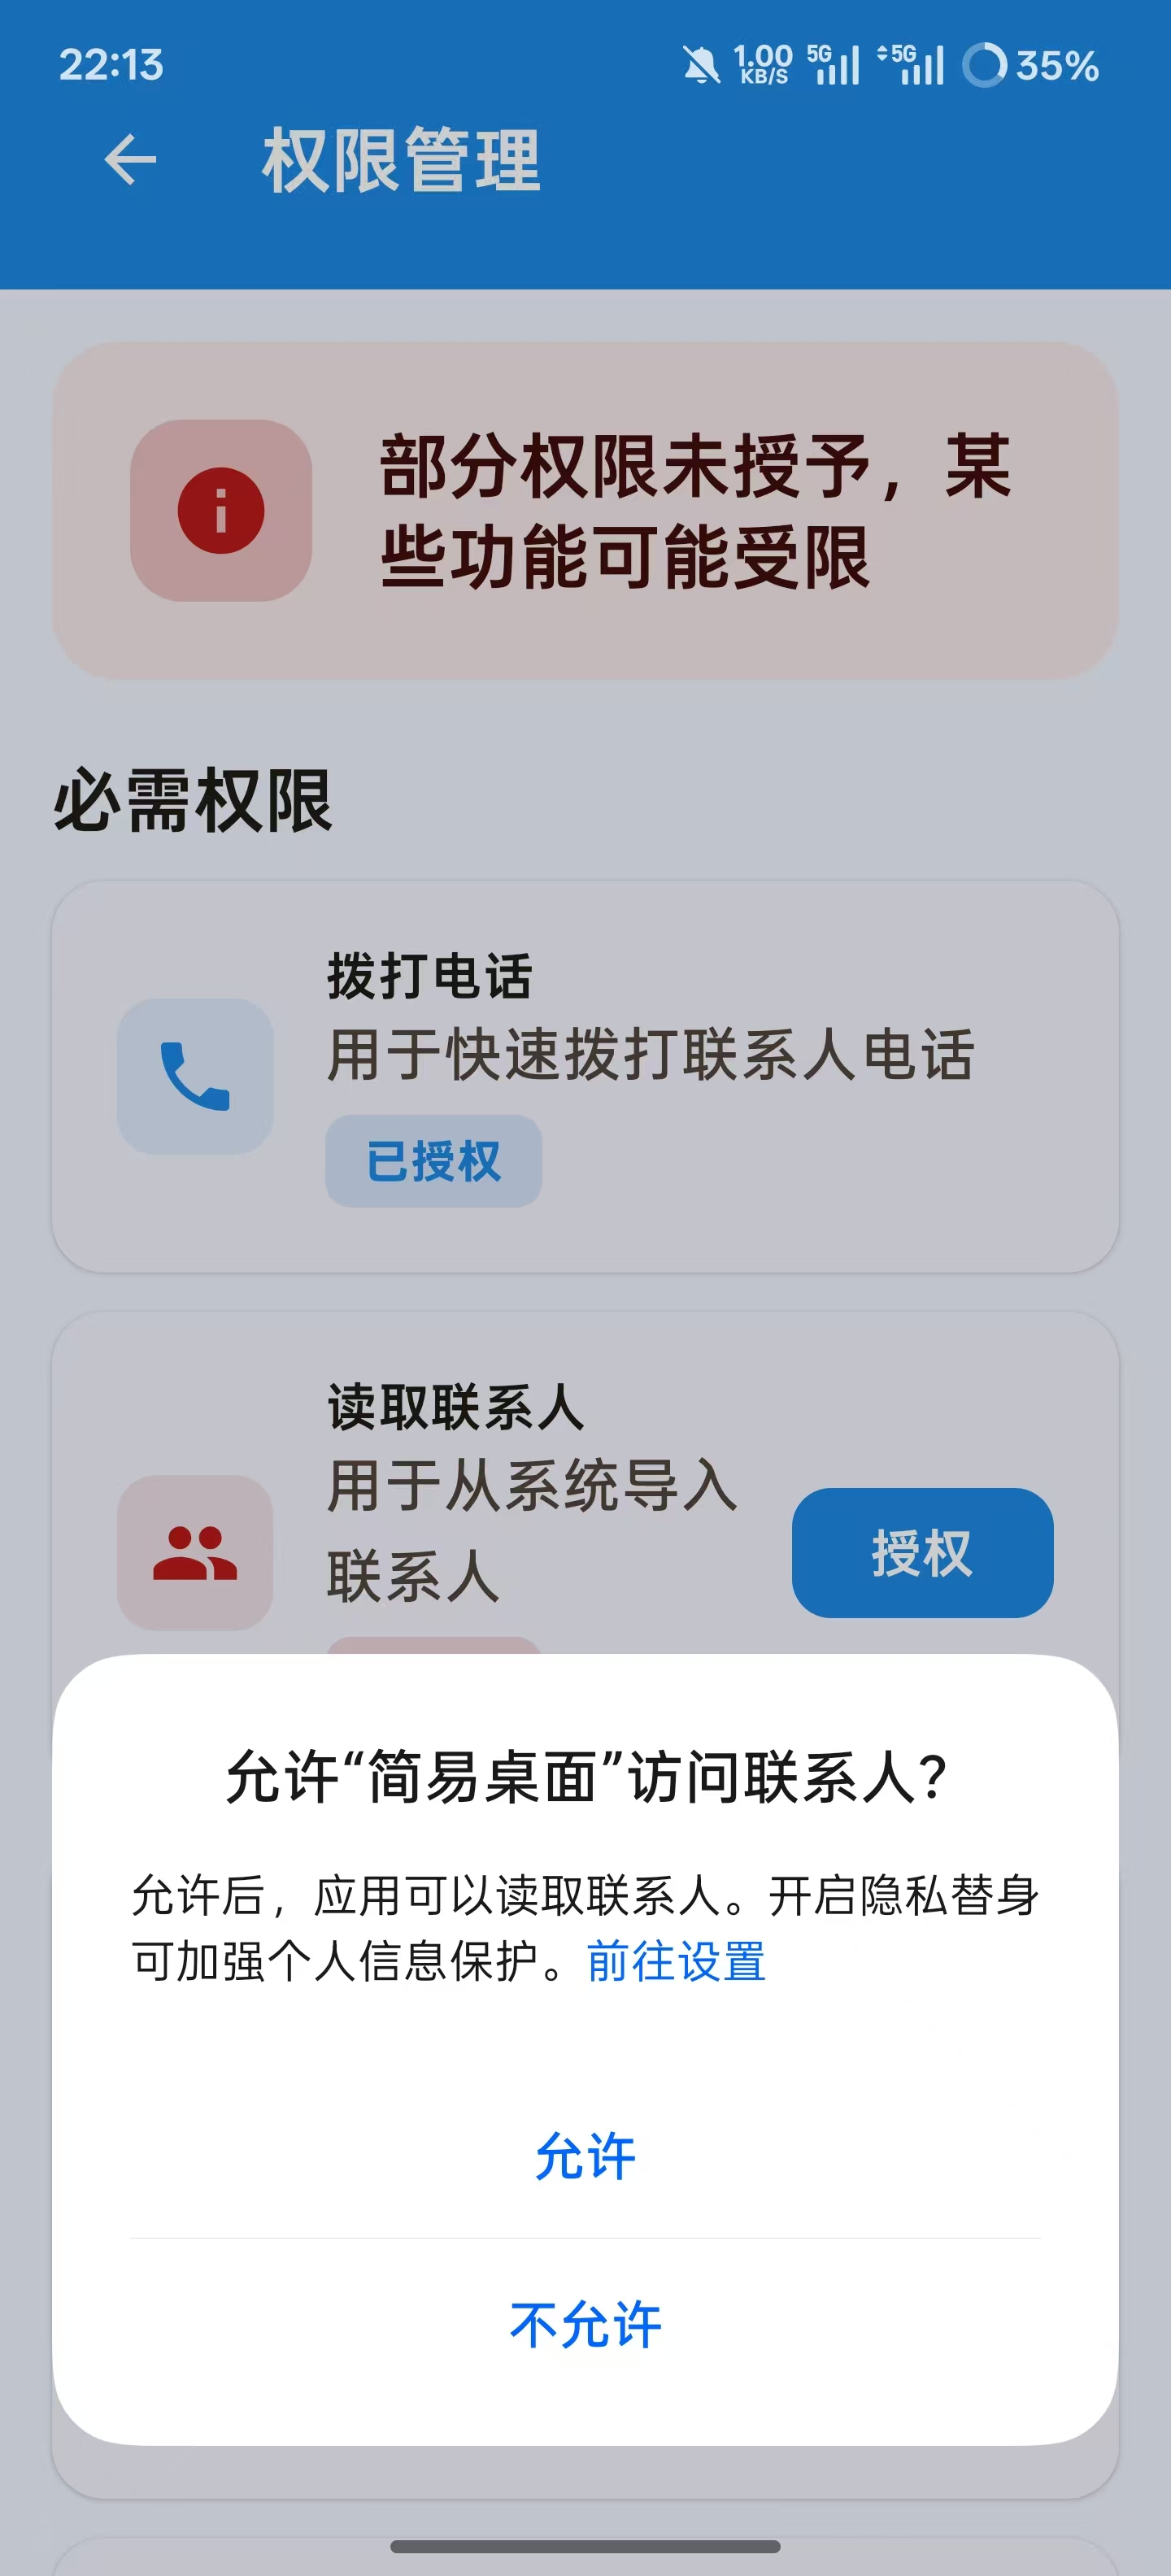
\includegraphics[width=\linewidth]{figures/wechat/desktop5.jpg}
        \caption*{(e) 权限设置}
    \end{minipage}\hfill
    \begin{minipage}{0.22\textwidth}
        \centering
        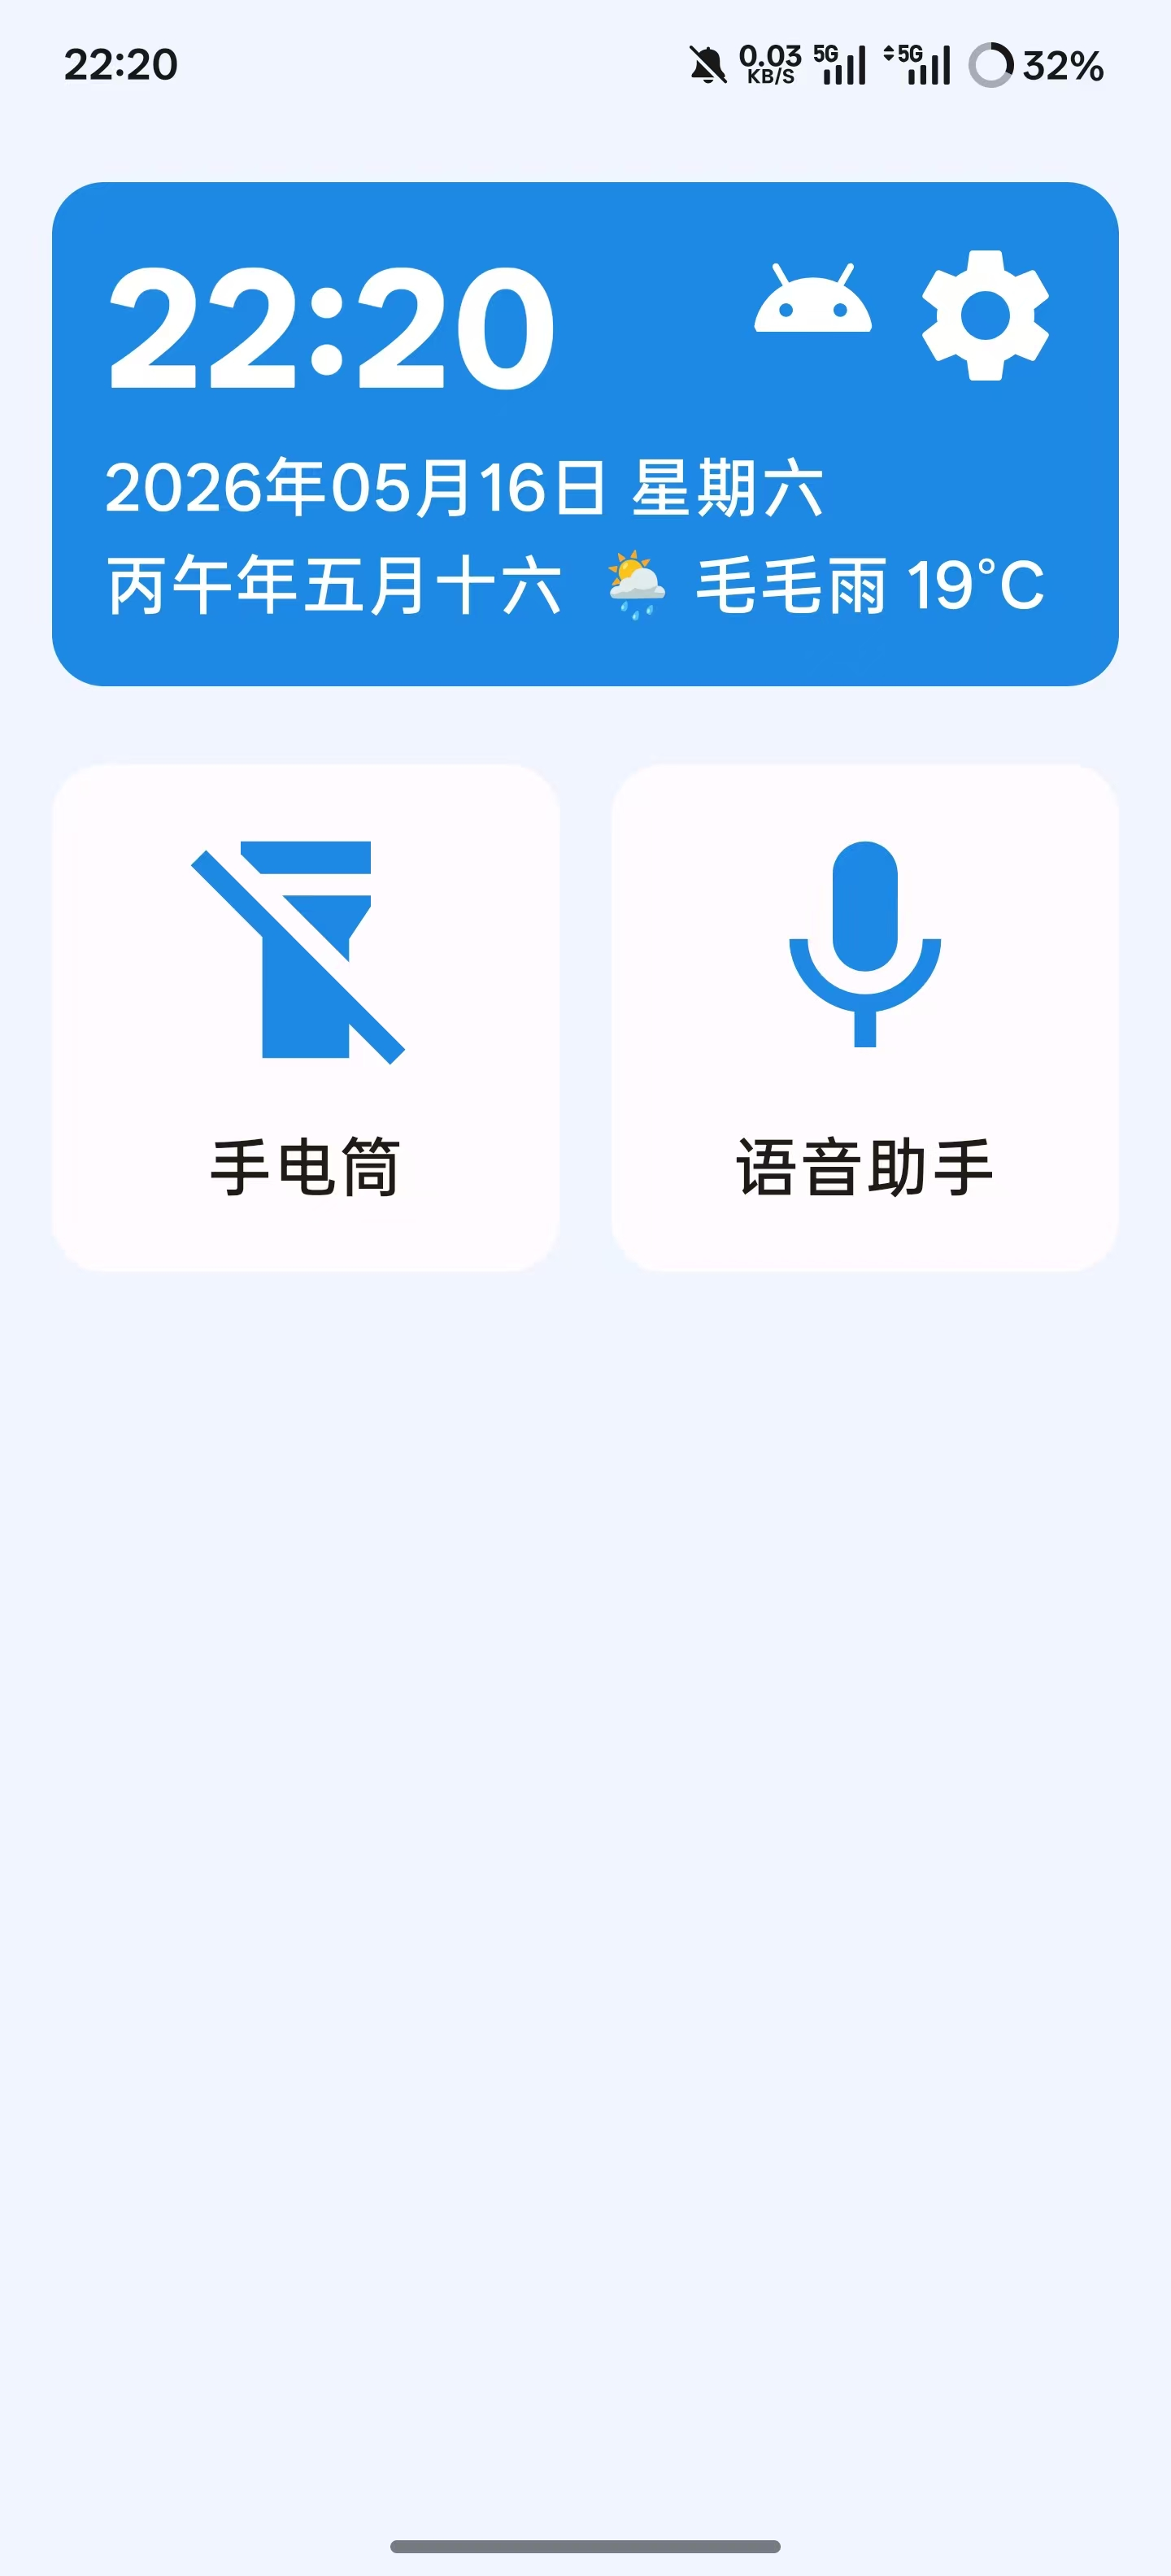
\includegraphics[width=\linewidth]{figures/wechat/desktop6.jpg}
        \caption*{(f) 初始主页}
    \end{minipage}
    \caption{SimpleDesktop 简易桌面首次启动页面}
    \label{fig:wechat_first_boot}
\end{figure}


滑动至最后一页时，引导页提供完成引导按钮，点击后系统自动跳转至权限申请页面，依次申请电话拨打权限、读取联系人权限、相机权限（用于拍摄头像）、位置权限（用于天气定位）等运行时权限。如果当前设备运行在Android 6.0及以上版本且尚未授权，系统会通过XXPermissions权限框架弹出系统级权限对话框；老年用户可在子女协助下完成授权操作。

权限授权完成后，系统提示用户开启无障碍服务\upcite{13}，这是微信一键直拨与WiFi自动开启功能的前置条件。系统通过专门设计的引导对话框图文并茂地说明授权步骤，并提供一键跳转到无障碍设置页的快捷入口。完成无障碍授权后，系统将自身设置为默认桌面应用，此时初始化流程结束，用户进入主屏。



\subsection{日常使用主流程}

在日常使用中，老年用户启动设备后直接进入SimpleDesktop主屏。主屏顶部实时显示当前时间、日期、农历和天气，让老年用户对当下信息一目了然。

\begin{figure}[htbp]
    \centering
    \begin{minipage}{0.22\textwidth}
        \centering
        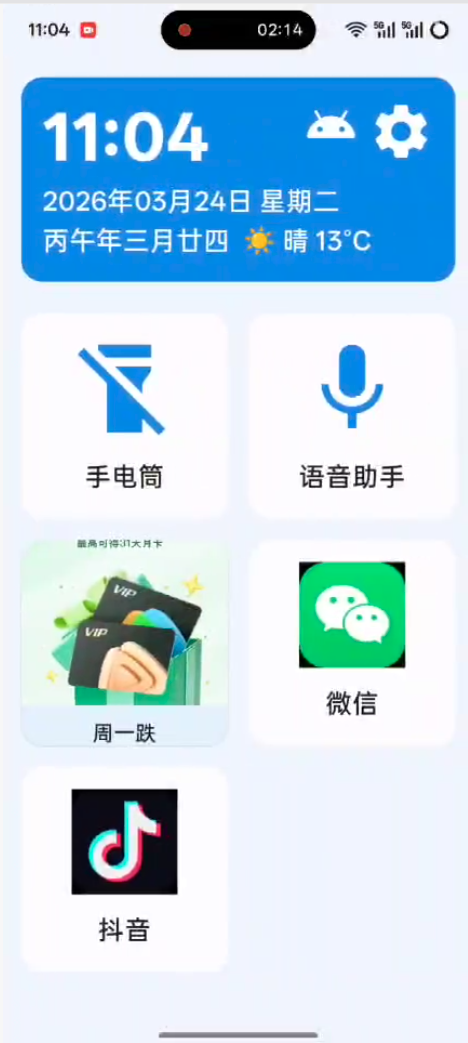
\includegraphics[width=\linewidth]{figures/demo1.png}
        \caption*{(a) 桌面触发状态}
    \end{minipage}\hfill
    \begin{minipage}{0.22\textwidth}
        \centering
        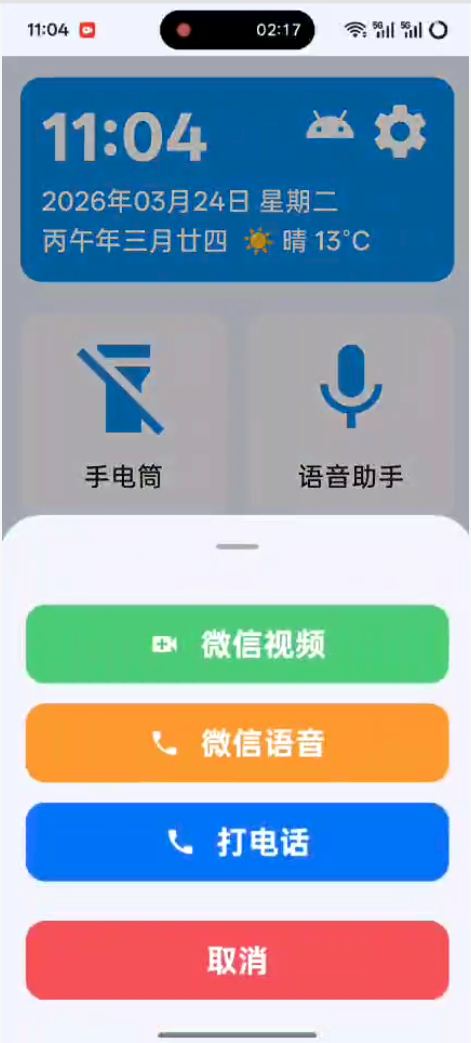
\includegraphics[width=\linewidth]{figures/demo2.png}
        \caption*{(b) 呼叫选项调起}
    \end{minipage}\hfill
    \begin{minipage}{0.22\textwidth}
        \centering
        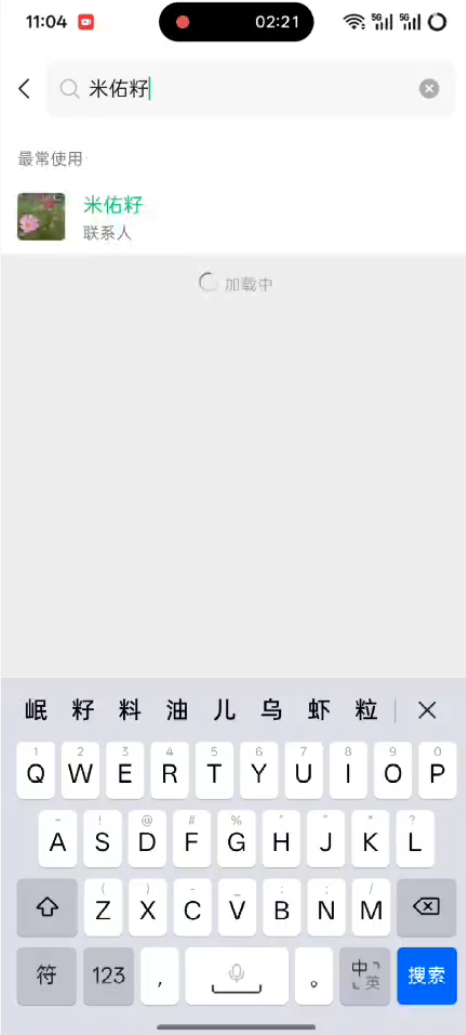
\includegraphics[width=\linewidth]{figures/demo3.png}
        \caption*{(c) 注入搜索匹配}
    \end{minipage}

    \vspace{0.4cm}

    \begin{minipage}{0.22\textwidth}
        \centering
        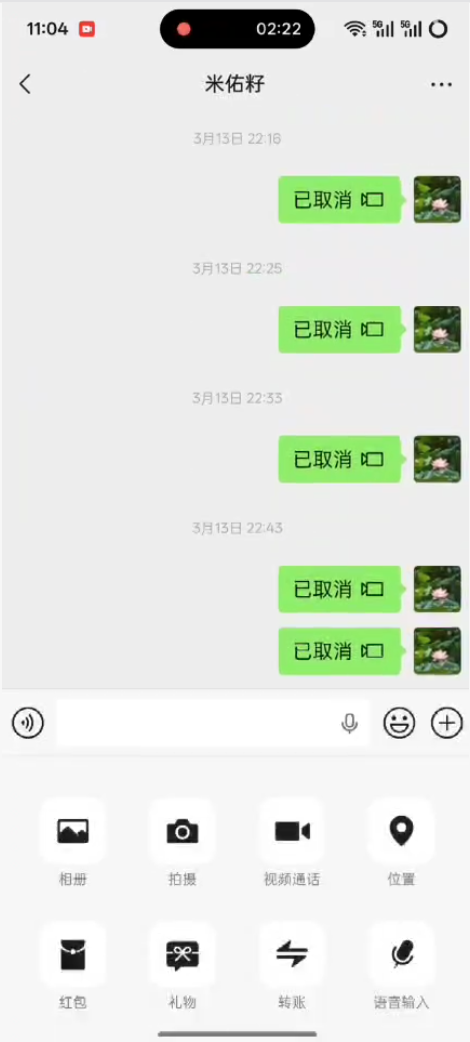
\includegraphics[width=\linewidth]{figures/demo4.png}
        \caption*{(d) 激活目标会话}
    \end{minipage}\hfill
    \begin{minipage}{0.22\textwidth}
        \centering
        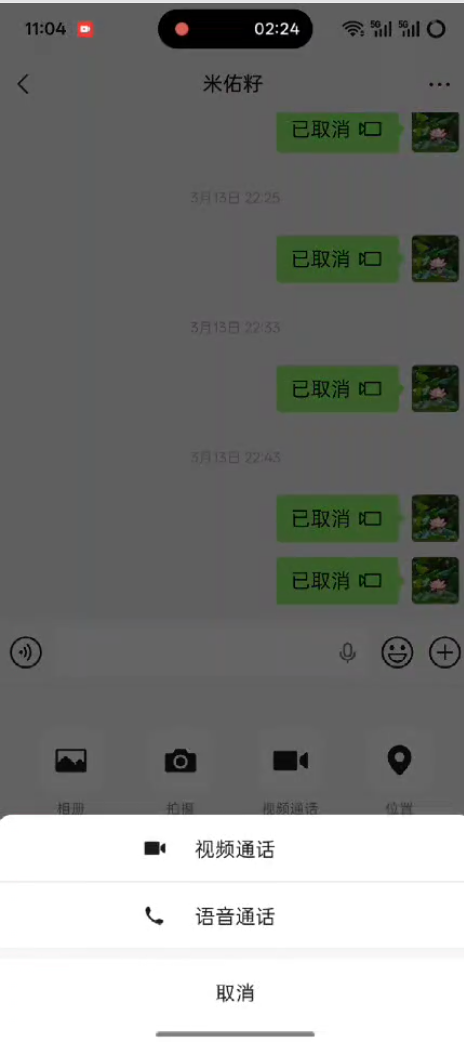
\includegraphics[width=\linewidth]{figures/demo5.png}
        \caption*{(e) 展开功能面板}
    \end{minipage}\hfill
    \begin{minipage}{0.22\textwidth}
        \centering
        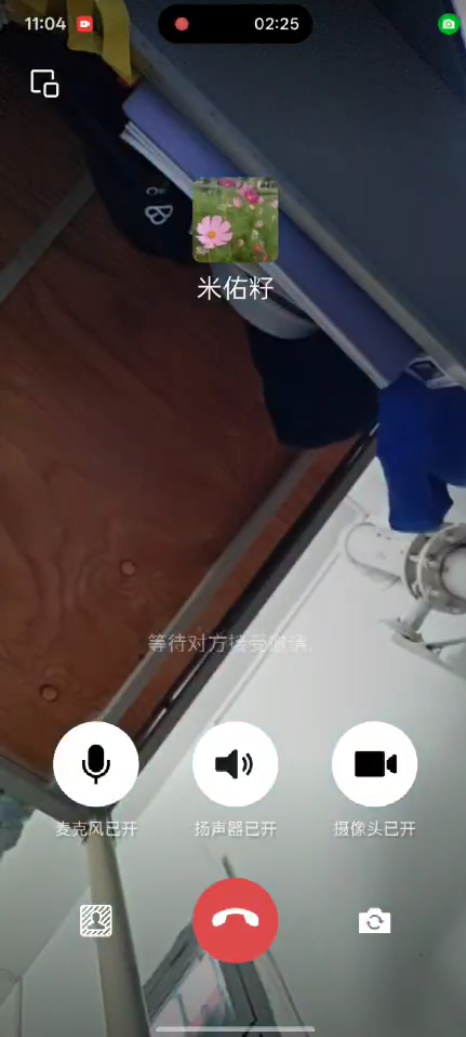
\includegraphics[width=\linewidth]{figures/demo6.png}
        \caption*{(f) 通话链路建立}
    \end{minipage}

    \caption{SimpleDesktop 微信自动化直连全过程状态机流转展示}
    \label{fig:wechat_fsm_process}
\end{figure}

当老年用户希望与某位亲友视频通话时，只需点击主屏上的对应联系人卡片。卡片底部弹出操作面板，呈现视频通话、语音通话、电话拨打三个清晰的大按钮（按钮的具体可见性根据该联系人配置的通话能力决定）。用户点击视频通话按钮后，系统自动启动微信，无障碍服务接管后续的七阶段自动化流程\upcite{16,17}，约5至6秒后自动进入与目标联系人的微信视频通话界面。

当老年用户希望使用某个应用时，从主屏向下滚动找到对应的应用卡片并点击，系统通过Android标准的Intent机制启动目标应用。常用应用列表可通过设置中心的应用管理界面进行自定义增删与排序。

当老年用户希望使用语音助手时，点击主屏上的语音助手卡片，弹出全屏的语音对话界面。界面顶部以大字号实时显示识别出的文字内容，识别完成后系统自动解析意图，将操作目标和置信度反馈给用户，确认无误后自动执行对应操作（拨打电话、发起微信通话或启动应用）。

\subsection{异常处理流程}

系统的异常处理流程主要覆盖网络异常和操作异常两类典型场景。网络异常方面，当WiFi连接突然断开时，前台守护服务立即触发自愈流程：启动无障碍服务自动操作WiFi开关\upcite{13}并跳转至系统WiFi设置页完成自愈。20秒宽限期内若网络成功恢复，整个过程对用户透明；若超时仍未恢复，系统弹出网络异常提示弹窗并播报语音提示，引导用户进行人工干预。

操作异常方面，微信自动化流程在遇到来电通知、系统弹窗等外部干扰时，焦点防冲突退避机制自动启动\upcite{13}，先关闭干扰窗口再继续执行流程；如果干扰持续时间过长，系统在多次重试后主动放弃当前指令并安全重置状态机，避免出现死锁，老年用户可在桌面上重新发起通话操作。

